% !TeX spellcheck = en_GB
\documentclass{template}

\usepackage{makros}



% metadata
\titlehead{\includegraphics[height=1.4cm]{rwth.pdf} \hspace{1cm}
%\includegraphics[height=1.4cm]{l2m-banner.jpg}
}

\subject{Master Thesis}
\title{Discontinuous Galerkin Methods for the \MA Equation}
\subtitle{\Large Discontinuous Galerking Verfahren zur Lösung der Monge-Amp\`ere-Gleichung}
\author{Elisa Friebel} %\\ Matrikelnummer: 295932
\date{\today}
\publishers{Gutachter: Prof. W. Dahmen\\ Prof. S. Noelle}

% begin document
\begin{document}


\pagenumbering{Alph}
% title page
\maketitle
%\cleardoublepage

% erklärung
\begin{center}
\begin{minipage}[t]{0.8\textwidth}

\chapter*{Erklärung}
Ich versichere hiermit, dass ich die vorliegende Arbeit selbständig und
ohne Benutzung anderer als der angegebenen Hilfsmittel angefertigt habe.
Alle Stellen, die wörtlich oder sinngemäß aus veröffentlichten und nicht
veröffentlichten Schriften entnommen sind, sind als solche kenntlich
gemacht.

\vspace{1cm}
Aachen, den \today

\vspace{2cm}
(Elisa Friebel)
\end{minipage}
\end{center}
\thispagestyle{empty}
\cleardoublepage

% toc
\pagenumbering{roman}
\tableofcontents{}

%\cleardoublepage
\setcounter{page}{1}
\pagenumbering{arabic}

% content

% warum wollen wir etwas tun?was wollen wir tun? welche kapitel gibt es?
%\chapter{Preface}
\label{ch:preface}

% wie sieht das mathematische modell aus?
\chapter{Mathematical foundations}
\label{ch:TheoreticalBackground}
This chapter discusses the mathematical foundation for the numerical schemes which are presented in later chapters.
At the beginning of this chapter we repeat the basic definitions and notation for an analysis of partial differential equations as they are introduced for example in \cite[Introduction]{Evans1998}. Afterwards we introduce the finite element, as well as a discontinuous Galerkin method, for the latter we provide also a proof of its well-posedness. To prepare later calculations we end this chapter with some algebraic identities about the Hessian.

\section{ Preliminaries and Notation}
Let $\Omega \subset \R^d $ be an open, bounded area and $\partial \Omega$ its boundary.
\begin{definition}[Partial Differential Equation{\cite[Introduction]{Evans1998}}]
 A \emph{partial differential equation} (PDE) of order $k\in \N$ is an expression of the form
\begin{align}
	F(D^k u(x), D^{k-1}u(x), \dots, Du(x), u(x), x) = 0, \; (x \in \Omega)\label{eq:general PDE}
\end{align}
where $F:\R^{n^k} \times \R^{n^{k-1}} \times \dots \times \R^n \times \R \times \Omega \rightarrow \R $ is given and $u:\Omega \rightarrow \R$ is unknown.
\end{definition}
We focus in this thesis on second-order PDEs for our main PDE, namely the \emph{\MA equation} which we will introduce later is of second order. 
\\Beside the order there exist further properties to categorise PDEs:
\begin{definition}[Categories of PDEs{\cite[Introduction]{Evans1998}}] \label{def: categories of PDEs}
	Given functions  $f:\Omega \rightarrow \R$ and $a_{\alpha}:\Omega \rightarrow \R$ or $a_{\alpha}:\R^{n^{k-1}} \times \dots \times \R^n \times \R \times \Omega$ respectively, for $\alpha \in \N^{k}, |\alpha| \leq k$, a PDE of order $k$ is called
	\begin{enumerate}[(i)]
		\item \emph{linear} if it can be written in the form
		\[
			\sum_{|\alpha| \leq k} a_{\alpha} (x) D^{\alpha} u(x) = f(x).
		\] 
		
%		\item \emph{semilinear} if it can be written in the form
%		\[
%			\sum_{|\alpha| = k} a_{\alpha}(x) D^{\alpha} u + a_0(D^{k-1}u, \dots, Du, u, x)= f(x),
%		\]	
%		i.e. a semilinear PDE is nonlinear in the unknown function, but linear in all partial derivatives.
		
		\item \emph{quasilinear} if it can be written in the form
		\[
			\sum_{|\alpha| = k} a_{\alpha}(D^{k-1}u, \dots, Du, u, x) D^{\alpha} u + a_0(D^{k-1}u, Du, u, x)= f(x),
		\]	
		i.e. a quasilinear PDE is nonlinear in (at least) one lower derivate, but linear in the highest order derivates.
		
		\item \emph{fully nonlinear} if it depends nonlinearly upon the highest order derivatives.
	\end{enumerate}
\end{definition}
The standard example for linear PDEs is the \emph{Poisson equation} $-\triangle u = f$.
% a semilinear PDE is for example the \emph{nonlinear Poisson equation} $-\triangle u = f(u)$.
A well-known example for quasilinear PDEs are equations of the type $\nabla \cdot (A(u) \nabla u) = f$, where $A: \R^d \rightarrow \R^{d \times d}  $. The \MA equation $\mydet {D^2 u} = f$ is part of the last category, the nonlinear PDEs. 

Another important property to classify second-order PDEs is ellipticity. 
\begin{definition}[Elliptic PDE{, \cite[p.207]{FGN2013}}]
	A fully nonlinear second order PDE is called \emph{elliptic} if its operator satisfies
	\begin{align}
		F(A,p,z,x) \leq F(B,p,z,x) \label{eq: ellipitic PDE}
	\end{align}
for all $x \in \Omega, z \in \R, p \in \R^d$ and $A,B \in \R^{d \times d}_{sym}$  with $A-B$ positive semidefinite.

%This notion is a natural extension of the ellipticity concept for first order PDEs. Interpreting a first order PDE operator as a function depending on $D^2u, Du, u, x$, \eqref{eq: ellipitic PDE} characterises an elliptic PDE.
\end{definition}

Searching for a function $u:\Omega \rightarrow \R$ with 
\begin{align}
u=g \text{ on } \partial \Omega \label{eq: boundary}
\end{align}
for some $g:\partial \Omega \rightarrow \R$ is called a \emph{Dirichlet-boundary problem}. The function $u:\Omega \rightarrow \R$ fulfilling \eqref{eq:general PDE} and \eqref{eq: boundary} is called a classical solution of the problem. 

There are problems such that no classical solution exists. A PDE of order $k$ requires its classical solution to be at least $k$ times differentiable, which is a very strong demand. To admit less regular solutions one aims for a weaker notion of a solution. Before doing this we specify some function spaces.

\begin{definition} [Function Spaces and Norms]\label{def: function spaces and norms}
Accordingly to the majority of the literature we refer by $W^{s,p}(\Omega)$ to the H\"older space, a set consisting of all $L^p(\Omega)$ functions whose distributional derivates up to order $s$ are contained in $L^ p(\Omega)$.
In the special case $p=2$ they are referred to as Sobolev spaces $H^s(\Omega):=W^{s,2}(\Omega)$. An additional subscript $0$ denotes the set where all functions are zero at the boundary, i.e. $H^s_0 :=\{f \in H^s(\Omega); f(x)=0 \; \forall x \in \partial \Omega\}$.

The corresponding function space norms are defined by
\[
	\norm f _{W^{s,p}(\Omega)} = \left( \sum_{|\alpha| \leq s} \norm{D^\alpha f}^p_{L^p(\Omega)}\right)^{\frac 1 p }, \text{   especially } \norm f _{H^{s}(\Omega)}=\left( \sum_{|\alpha| \leq s} \norm{D^\alpha f}^2_{L^2(\Omega)}\right)^{\frac 1 2 }
\]
and the $H^s$ semi-norms
\[ 
 	|f|_{H^{s}(\Omega)}=\left( \sum_{|\alpha| = s} \norm{D^\alpha f}^2_{L^2(\Omega)}\right)^{\frac 1 2 }.
\]
%If not stated otherwise $\bilin f g$ always refer to the standard $L^2$ scalar product 
%\[
%	\bilinLTwo{f}{g} = \myInt_{\Omega } f g.
%\]
For a normed function space $X$ we denote its dual by $X'$ and by $\bilin{\cdot}{\cdot}$ the pairing between $X$ and $X'$.

\end{definition}
By this definition it is clear that the $H^0$ norm and the $L^2$ norm conincide. 

Let $T$ be the triangle in $\Omega$ spanned by the points $v_0, v_1, v_2$. We also write 
\[
	T= \langle v_0, v_1, v_2 \rangle := \{\beta_0 v_0+ \beta_1 v_1 +\beta_2 v_2; \sum_{i=0}^2 \beta_i =1, \beta_i \geq 0, i= 0,1,2\}.
\]
We define the \emph{diameter} $diam(T)$ of a triangle $T$ as the diameter of the smallest circle containing $T$.

To discretise our domain $\Omega$ we subdivide it into simplices, more precisely we divide it into triangles.
\begin{definition}[Triangulation, {\cite[Definition 5.1]{Braess2003}}]
	We call a finite partition of $\Omega$ into triangles $\{T_1, \dots, T_n\}$ a feasible \emph{triangulation} $\mathcal{T}$, such that
	\begin{enumerate}[(i)]
		\item	$\overline \Omega = \bigcup_{T \in \triang} T$
		\item If $T_i \cap T_j$ is a point for $i \neq j$ , it is a vertex of both $T_i$ and $T_j$.
		\item If $T_i \cap T_j$ is more than one point for $i \neq j$, it is an edge of both $T_i$ and $T_j$.
	\end{enumerate}
	Let $h$ denote the maximal diameter $h:= \operatorname{max}\limits_{T\in \mathcal T} diam(T)$ in the triangulation $\mathcal T$, we then also refer to $\mathcal{T}$ by $\triang$. We call a triangulation \emph{regular} if every element is congruent.
\end{definition}
Note that this definition requires $\Omega$ to be a polygonal domain. However, there are extensions to domains with curved boundaries: In those triangles lying at the boundary are replaced by \quoting{triangles} which have curved sides. 

\begin{figure}[H]
\usetikzlibrary{calc}

		\begin{center}
		\begin{tikzpicture}[scale = 5]
%define coordinates
			\coordinate (vEins) at (0,0) ;
			\coordinate (vZwei) at (0:4cm);
			\coordinate (vDrei) at (90:4cm);

%draw square
			\draw (0,0) -- (1,0) -- (1,1) -- (0,1) -- cycle; 

%draw diagonals
			\draw (0,0) -- (1,1);
			\draw (1,0) -- (0,1);

			\draw (0.5,0) -- (1,0.5) -- (0.5,1)-- (0,0.5) --cycle; 

			\draw(0.25,0.25) -- (0.75,0.25) -- (0.75,0.75)-- (0.25,0.75) --cycle; 

			\draw node at (0.15,0.5) {$T_0$};

			\draw[color=blue, thick] (0.25,0.25)-- node[above]{\blue{$e_0$}} (0,0.5);
			\coordinate (vMiddle) ($(0.25,0.25)!0.5!(0,0.5)$);
			
			\draw[color=blue, thick, ->] ($(0.25,0.25)!0.5!(0,0.5)$) -- node[right=0.3, below=0.1]{\blue{$\mathbf n_{e_0}^{ T_0}$}} ($ ($(0.25,0.25)!0.5!(0,0.5)$) - (0.075,0.075)$);

		\end{tikzpicture}
		\end{center}

\caption{A regular triangulation of the unit square}
 \label{fig: triangulation}
\end{figure}

Figure \ref{fig: triangulation} shows a triangulation of the unit square. Since the edges uniquely define a triangulation of $\Omega$, we later also use the terms grid and mesh to refer to a subdivision into triangles.
An edge $e$ is called an interior edge if $e=T^+ \cap T^-$ holds for some $T^+,T^- \in \triang$, whereas it is called a boundary edge if $e \subset \partial \Omega$.
We divide the edges $\edges$ into the subsets $\edgesi$ and $\edgesb$ containing all interior edges and boundary edges, respectively. 
When we refer to a normal of an edge we always refer to an outward directed normal of one of the adjacent triangles. If it is not clear from the context to which triangle is referred we clarify that with a superscript.

On this basis we define some piecewise spaces.
\begin{definition}[Broken Spaces]
We define function spaces associated to a triangulation $\triang$ by
\begin{align*}
	H^s(\Omega;\triang) &:= \{f \in L^2(\Omega); f|_T \in H^s(T) \text{ for every } T \in \triang\}, \\
	\text{and }
	W^{s,p}(\Omega;\triang) &:= \{f \in L^p(\Omega); f|_T \in H^s(T) \text{ for every } T \in \triang\}.
\end{align*}	
\end{definition}

\begin{definition}[Piecewise Polynomial Spaces] \label{def: piecewise polySpace}
	Further we denote the finite-dimensional space of piecewise polynomials by
\[	
	\mathcal P^k_h = \{ f \in L^2(\Omega); f \arrowvert_T \textnormal{ is a polynomial of (total) degree } \leq k \textnormal{ for every } T \in \triang\}.
\]
\end{definition}

For later analysis we need the approximation properties of $\mathcal P_h^k$ proven in \cite[Chapter 4]{BS2002}, as well as standard trace and inverse estimates as proven in \cite[Section 1.6 and Section 4.5]{BS2002}.
\begin{lemma}[Approximation properties of $\mathcal P_h^k${,\cite[Theorem(4.4.20)]{BS2002}}]  \label{la: approximation properties}
Let $s,m \in \N$ with $0 \leq m \leq s\leq k+1$. Then for any $u \in H^s(\Omega)$, there exists $v_h \in \mathcal P^k_h$ such that 
\[
	\left( \sum_{T \in \triang} \norm{u-v_h}^2_{H^m(T)} \right)^{\frac 1 2} \leq C h^{s-m} \norm{u}_{H^{s}(\Omega)},
\]
where $C$ is a constant depending only on the mesh, but not in $h$ or $u$.
\end{lemma}
\begin{lemma}[Trace estimate{,\cite[Theorem(1.6.6)]{BS2002}}]\label{la: trace estimate}
	Given any quasi-uniform trianguliaton $\triang$, there holds for $ v \in H^1(\Omega;\triang)$
	\begin{align*}
	%	\norm{v}_{L2 (\partial T)}^2 \leq C\left(\frac 1 {h_T} \norm{v}_{L2(T)}^2  + h_T \norm{\nabla v}_{L2(T)}^2\right) \qquad \forall v \in H^1(T).
	\sum_{e \in \edges} \LTwonormE{v}^2 
		\leq C_1
		 \sum_{T \in \triang} \LTwonormT{v} \HOnenormT{v}
	\leq 
		C_2 \sum_{T \in \triang} \left(\frac 1 {h} \LTwonormT{v}^2  + h \HOnenormT{v}^2\right).
	\end{align*}
	 where $C_1,C_2$ are positive constants depending only on the mesh but not on $v$.
\end{lemma}
Note that the second inequality follows from Young's inequality $\sqrt{a} \sqrt{b} \leq \varepsilon a + \frac 1 \varepsilon b$ for arbitrary $a,b \in \R^+$ and $\varepsilon \geq 0$. This inequality can be easily verified taking the root of the inequality $ab \leq \varepsilon^2 a^2 + 2ab + {\frac 1 \varepsilon}^2b^2 = \left( \varepsilon a + \frac 1 \varepsilon b\right)^2$.

\begin{lemma}[Inverse Estimate{, \cite[Lemma 2.4]{BGN+2011}}]\label{la: inverse estimate}
	For any piecewise polynomial $v \in \mathcal P_h^k$ there holds
	\[
	\norm v_{H^m(T)} \leq C h^{s-m} \norm v_{H^s(T)} \qquad \forall T \in \triang
	\]
\end{lemma}

To formulate a method capable of handling discontinuities along triangle edges we introduce edge operators.   
\begin{definition}[Edge Operators] \label{def: edge operators}
We denote the \emph{normal jump} of  a piecewise smooth function $u_h:\Omega \rightarrow \R$ across an edge $e \in \edges$ by
\begin{align*}
	\jump {u_h}&:= 
	\begin{cases}
		u_h^+  \mathbf n^+ + u_h^- \mathbf n^-  &\text{ if } \partial T^+ \cap \partial T^- = e \text{ for some }T^+,T^- \in \triang, \\
		u_h \mathbf n 	 &\text{ if } \partial T \cap \partial \Omega = e \text{ for some } T \in \triang,
	\end{cases}	
\end{align*}
where $n^\pm$ are the normals with respect to $T^\pm$ and  $u_h^\pm(x) := \lim_{\varepsilon \rightarrow 0} u_h(x-n^\pm \varepsilon)$.
Likewise we define the normal jump of a piecewise smooth function $u_h:\Omega \rightarrow \R^2$ across an edge $e \in \edges$ by
\begin{align*}
	\jump {u_h}&:= 
	\begin{cases}
		u_h^+ \cdot \mathbf n^+ + u_h^-\cdot  \mathbf n^-  &\text{ if } \partial T^+ \cap \partial T^- = e \text{ for some }T^+,T^- \in \triang,\\
		u_h\cdot \mathbf n 	 &\text{ if } \partial T \cap \partial \Omega = e \text{ for }T\in \triang.
	\end{cases}	
\end{align*}
Here $\cdot$ denotes the scalar product.
Note that the jump of a scalar is a vector, whereas the jump of a vector is a scalar.

The \emph{average} of a piecewise smooth function $u_h:\Omega \rightarrow X$ for every $X$ across an edge $e \in \edges$ is defined by
\begin{align*}
	\average {u_h} &:= 
	\begin{cases}
	\frac 1 2 \left(u_h^+ + u_h^-\right) &\text{ if } \partial T^+ \cap \partial T^- = e \text{ for some }T^+,T^- \in \triang, \\
	 u_h &\text{ if } \partial T \cap \partial \Omega = e \text{ for }T\in \triang.
	\end{cases}
\end{align*}
\end{definition}

We end this section with the note that we use a subscript $h$ to indicate a piecewise evaluation or interpretation.  Subsequently differential operators with a subscript $h$ imply that differentiations were carried out seperately on every triangle, for example the piecewise gradient is defined by $\nabla_h f |_T = \nabla f |_T \; \forall T \in \triang$. 



\section{Finite Element Method}
Before we discuss numerical schemes for the \MA equation we shortly recall how a finite element method works, for a deeper insight in finite element methods we recommend \cite{Braess2003, BS2002}. Since the finite element method bases on a variational formulation we introduce the method talking about the well-known example of the generalised Poisson equation. 

%\subsection{The Poisson Problem}

\begin{definition}[Generalised Poisson Problem] \label{def: General Poisson Problem}
The \emph{generalised Poisson problem} is finding a function $u:\Omega \rightarrow \R$ such that 
\begin{align}
	-\nabla \cdot (A \nabla u) = f \qquad &\text{ in }\Omega \label{eq: poisson eq} \\
	u = g \qquad &\text{ on } \partial \Omega    \label{eq: poisson bc}
\end{align}
for $ A:\Omega^d \rightarrow \R^{d \times d}$ symmetric and functions $f,g:\Omega \rightarrow \R $. 
Because of the physical context of this PDE the matrix $A$ is also referred to as \emph{diffusion matrix}.
\end{definition}

First, we note that we can reduce all general Poisson problems with Dirichlet boundary data to problems with \emph{homogeneous boundary data}, i.e. $g(x) = 0$ for all $x \in \partial \Omega$: Let us assume $\tilde g$ is defined on all of $\Omega$ with $\tilde g = g$ on $\partial \Omega$. Due to the linearity of the differential operators we have that $v:=u-\tilde g$ satisfies
\begin{align}
	-\nabla \cdot (A \nabla v) &= f + \nabla \cdot (A \nabla \tilde g)  \qquad &&\text{ in }\Omega \label{eq: poisson homogeneous eq} \\
	v &= 0 \qquad &&\text{ on } \partial \Omega.    \label{eq: poisson homogeneous bc}
\end{align}
Hence, we can restrict ourselves to the case with homogeneous boundary data.

We are now able to set up a \emph{weak formulation} of the generalised Poisson problem based on variational principles, this formulation is the key element for deriving a finite element method.

Due to the main theorem of variational analysis every classical solution to \eqref{eq: poisson eq} fulfils 
\begin{align}
	-\myIntX \Omega {\varphi \nabla \cdot (A \nabla u)}=
	 \myIntX \Omega {\varphi f} \qquad \forall \varphi \in C_0^\infty(\Omega), \label{eq: variational form}
\end{align}
and vice versa.
Integration by parts yields to
\begin{align*}
	\myIntX \Omega {\nabla \varphi  \cdot A\nabla u}
		%-\myIntS  {\partial \Omega} { \varphi (A\nabla u) \mathbf{n} }
	= \myIntX  \Omega { \varphi f } \qquad \forall \varphi \in C_0^\infty(\Omega). %\label{eq: FE integration by parts}
\end{align*}
The last statement can be reformulated to the so called variational form 
\begin{align}
a(\varphi,u)  = b(\varphi) \qquad \forall \varphi \in C_0^\infty(\Omega). \label{eq: variational formulation}
\end{align}
with the bilinear form $a:C_0^\infty(\Omega) \times X \rightarrow \R$
\begin{align*}
a(\varphi,u) = \myIntX  \Omega { \nabla \varphi  \cdot A\nabla u }
	% -\myIntS  {\partial \Omega} { \varphi (A\nabla u) \mathbf{n}}
\end{align*}
where $X$ is a function space we define in a moment and the functional $b:C_0^\infty(\Omega) \rightarrow \R$
\begin{align*}
 b(\varphi)  = \myIntX  \Omega { \varphi f}.
\end{align*}


\begin{definition}[Weak Solution]
	Functions satisfying \eqref{eq: variational formulation} are called \emph{weak solutions} of \eqref{eq: poisson eq}.
\end{definition}
Note that due to the lack of regularity weak solutions may not be restricted to the boundary of $\Omega$. However one can reformulate boundary conditions for weak solution with trace operators \cite[Section 5.5]{Evans1998}.

The generalised Poisson problem is well-posed in the sense that it has a unique weak solution if $A$ is positive definite and $f\in L^2(\Omega)$. This is mainly due to the ellipticity of the PDE (and as a consequence thereof the ellipticity of $a$). Thus, it is possible to apply the Lax-Milgram theorem and a maximum principle. For an analysis we refer the interested reader to \cite[Chapter~6]{Evans1998}.

On the left-hand side in the weak notation only first derivatives of $u$ appear, hence \eqref{eq: variational formulation} is also applicable for functions $u$ which are not twice differentiable. It turns out that the previously defined Sobolev spaces are well-suited candidates for the space $X$ containing weak solutions \cite[Chapter 1]{BS2002}. Therefore we search for the solution of the infinite-dimensional problem: Find $u\in H_0^1(\Omega)$ such that  $a(\varphi,u)  = b(\varphi) \;\forall \varphi \in C_0^\infty(\Omega)$ holds. % $\forall \varphi \in C^\infty(\Omega)$.

The main idea of the finite element method is to approximate the two function spaces, namely the spaces $H_0^1(\Omega)$ and $C_0^\infty(\Omega)$ containing $\varphi$ and $u$, respectively by finite dimensional spaces $W_h$ and $V_h$. For those spaces should hold a analogous equation as we have in the variational form stated in \eqref{eq: variational formulation}.

The finite space $W_h$ is called \emph{test space} and its elements are called \emph{test functions}. $V_h$ is referred to as \emph{ansatz} or \emph{trial space}, the contained functions accordingly \emph{ansatz} or \emph{trial functions}. According to the boundary conditions of the original function spaces we demand for the finite spaces that $u_h|_{\partial \Omega} = 0$ for every $u_h \in V_h \cup W_h$.

Usually these limited function spaces are based on a discretisation of $\Omega$ and are only piecewise smooth. Consequently, we have to replace all operators appearing in $a$ by operators defined on $W_h \cup V_h$. We denote these discretised versions using the subscript $h$.

With these preliminaries we can define the finite element methods as searching for $u_h \in V_h$ such that 
\begin{align}
a_h(w_h,u_h) = b_h(w_h) \qquad \forall w_h \in W_h. \label{eq: FE variational formulation}
\end{align}
with the bilinearform  $a_h:W_h \times V_h \rightarrow \R$
\begin{align*}
a_h(w_h,u_h)  = \myIntX  \Omega { \nabla w_h  \cdot A\nabla u_h} %-\myIntS  {\partial \Omega} { w_h (A\nabla u_h) \mathbf{n}}
\end{align*}
and the function $b:W_h \rightarrow \R$
\begin{align*}
b_h(w_h) = \myIntX  \Omega { w_h f}.
\end{align*}

This general proceeding is called a \emph{Galerkin approach}. Choosing $W_h = V_h$ yields to the so-called \emph{Galerkin methods}, otherwise the methods are referred to as \emph{Petrov-Galerkin methods}.

To construct $u_h$ we first choose a basis $B_W$ of $W_h$ and a basis $B_V$ of $V_h$.
Since the left-hand side is linear in $w_h$ we only need to check the equations in \eqref{eq: FE variational formulation} for all $w_h \in B_W$. 
Furthermore we can express $u_h$ as the linear combination of basis functions, namely $\sum_{p \in B_V} \mathbf{c}_p \; p$ and hence, we can rewrite \eqref{eq: FE variational formulation} as a linear system of equations $M \mathbf{c} = \mathbf{b}$ where  $\mathbf{c}$ is the unknown coefficient vector of $u_h$ to the basis $B_V$.  The matrix $M$ sometimes is named the \emph{system} or \emph{stiffness matrix}.

Altogether a finite element method for the generalised Poisson equation is defined by the bilinearform $a$ and the functional $b$ together with the choice of $W_h$ and $V_h$. Its computations consist of the assembling process where the matrices $M$ and the right-hand side vector $b$ are computed and the solving process of the resulting linear system of equations.\\
The error made by restriction to finite elements is characterised by the following Lemma.
\begin{lemma}[C\'ea Lemma{, \cite[(2.8.5)]{BS2002}}] \label{la: Ceas lemma}
	Let the bilinear form $a$ be $V$ elliptic with $H_0^m \subset V \subset H^m(\Omega) $, i.e. $0 < \alpha \leq C$ exist with
	\[
		a(u,u) \geq \alpha  \norm u ^2_V \text{ and } |a(v,u)| \leq C \norm u _V \norm v _V.
	\]
	Then for the solution $u_h$ of \eqref{eq: FE variational formulation}  holds
	\begin{align}
		\norm {u - u_h}_V \leq \frac C {\sqrt \alpha} \inf\limits_{v_h \in V_h} \norm {u-v_h}_V.
	\end{align}
\end{lemma}
This result shows that the quality of the finite element solution depends on the one hand on the problem parameters $\alpha$ and $C$, but on the other hand particularly on the approximation properties of $V_h$. A typical choice for the function spaces $W_h$ and $V_h$ are piecewise polynomials spaces which have good approximation properties and are easy to handle.

\section{Discontinuous Galerkin} \label{sec: SIPG}
A recent idea is to to include discontinuous functions when choosing the test and ansatz spaces. This approach arose in the context of hyperbolic PDEs whose solutions eventually contain discontinuities, later it was also applied to elliptic PDEs \cite{ABC+2002}. Although the generalised Poisson problem is not hyperbolic and its solutions are continuous we use this example to explain the issues arising when the finite element spaces are extended to discontinuities. The crux is the handling of function evaluations along discontinuities. Note that for discontinuous ansatz spaces it is no longer true that they are subspaces of $H_0^1(\Omega)$ which contains the weak solution of the generalised Poisson problem. That implies that C\'eas Lemma \ref{la: Ceas lemma} is not valid. Elements which include ansatz space not contained in $H_0^1(\Omega)$ are also referred to as non-conforming elements.

%We recall our triangulation $\mathcal{T}_h$ of $\Omega$. 
If we modify the derivation of the bilinear form defining the finite element method we can develop bilinear forms defined on the function space $V_h = \mathcal P_h^k$ (cf. Definition \ref{def: piecewise polySpace}). The method that we derive asserts the boundary conditions not by the choice of function spaces but force them implicitly in the bilinear form. Hence, we do not assume necessarily homogeneous boundary conditions anymore.

Due to the fact that we have discontinuities only along edges we perform the integration by parts in \eqref{eq: variational form} piecewise on every triangle leading to
\begin{align}
	a(v, u) = & \sum_{T \in \triang} \myIntX T {\nabla v \cdot A \nabla u }
		- \sum_{T \in \triang} \myIntS  {\partial T} { v A \nabla u \cdot \mathbf n}.
\end{align}
Since two adjacent elements share the same edge only with opposite directed normal vectors we can rewrite the last term as
\begin{align*}
\sum\limits_{T \in \triang}\myIntS  {\partial T} { v A \nabla u \cdot \mathbf n }
= &\sum\limits_{e \in \edgesi}\myIntS e { \left( v^+ A^+ \nabla u^+ \cdot \mathbf n^+ + v^- A^- \nabla u^- \cdot \mathbf n^- \right)} \\
& + \sum\limits_{e \in \edgesb}\myIntS e { v A \nabla u \cdot \mathbf n},
\end{align*}
where $h^\pm $ is $h$ evaluated in one of the two adjacent elements $T^\pm$ with $T^+ \cap T^- = e$. With the identity $\mathbf n^- = -\mathbf n^+$ we can extend
\begin{align*}
	&v^+ A^+ \nabla u^+ \cdot \mathbf n^+ + v^- A^- \nabla u^- \cdot \mathbf n^- \\
		= & \phantom{+} v^+ A^+ \nabla u^+ \cdot \mathbf n^+ 
		     + \frac 1 2  v^+ A^- \nabla u^- \cdot \mathbf n^- + \frac 1 2 v^+ A^- \nabla u^- \cdot \mathbf n^+ \\
		& + \frac 1 2  v^- A^+ \nabla u^+ \cdot \mathbf n^+ + \frac 1 2 v^- A^+ \nabla u^+ \cdot \mathbf n^-
		   + v^- A^- \nabla u^- \cdot \mathbf n^-.
\end{align*}
Splitting up first and last term, we find this equals to
\begin{align*}
		 & \phantom{+} \frac 1 2 v^+ A^+ \nabla u^+ \cdot \mathbf n^+ 
		     + \frac 1 2  v^+ A^- \nabla u^- \cdot \mathbf n^- + \frac 1 2  v^- A^+ \nabla u^+ \cdot \mathbf n^+ + \frac 1 2 v^- A^- \nabla u^- \cdot \mathbf n^- \\
		& + \frac 1 2  v^+ A^+ \nabla u^+ \cdot \mathbf n^+  + \frac 1 2 v^+ A^- \nabla u^- \cdot \mathbf n^+ +\frac 1 2 v^- A^+ \nabla u^+ \cdot \mathbf n^- + \frac 1 2 v^- A^- \nabla u^- \cdot \mathbf n^-\\
		    	  = & \phantom{+} \frac 1 2 \left(v^+ + v^- \right) \left(A^+ \nabla u^+ \cdot \mathbf n^+ + A^- \nabla u^- \cdot \mathbf n^- \right) \\
  &+  v^+ \frac 1 2  \left(A^+ \nabla u^+ + A^- \nabla u^-\right) \cdot \mathbf n^+ + v^- \frac 1 2 \left(A^+ \nabla u^+ + A^- \nabla u^-\right) \cdot \mathbf n^- \\
  = &  \jump {\average v  A \nabla u}+ \jump {v \average{ A \nabla u}}.
\end{align*}
Therefore the weak formulation can be written as $a(v,v) = l(v)$ with 
\begin{align*}
  a(v, u) = & \sum\limits_{T \in \triang} \myIntX  T { \nabla v \cdot A \nabla u} \\
	& - \sum\limits_{e \in \edgesi}\myIntS {e} {\left( \jump {\average v A \nabla u} + \jump {v \average{ A \nabla u}} \right)}\\
& - \sum\limits_{e \in \edgesb}\myIntS {e} {v A \nabla u \cdot \mathbf n}
\end{align*}
and
\[
l(v) = \sum_{T \in \triang} \myIntX  T { v f}.
\]
Due to the smoothness of the exact solution $u$ we neglect the jump in $A \nabla u$, i.e. $\jump A \nabla u =0$, and find
\begin{align*}
 a(v, u) = & \sum\limits_{T \in \triang} \myIntX  T { \nabla v \cdot \left(A \nabla u\right)} %\\
	- \sum\limits_{e \in \edgesi} \myIntS e {\jump{ v \average{ A \nabla u}}} %\right)
	\\
& - \sum\limits_{e \in \edgesb}\myIntS e { v A \nabla u \cdot \mathbf n}.
\end{align*}

To get a symmetric system matrix we symmetrise our bilinear form $a$ by adding terms. 
The first term we add is  $- \sum\limits_{e \in \edgesi}\myIntS e { \jump{ u \average{ A \nabla v}}}$ which equals zero when evaluating the integral for a smooth $v$. Hence it will vanish for the solution of the generalised Poisson problem. The second term required to achieve symmetry is  $-\sum\limits_{e \in \edgesb}\myIntS e { u A \nabla v \cdot \mathbf n}$. Since the Dirichlet boundary condition gives us solution values at the boundary this term equals $\sum\limits_{e \in \edgesb}\myIntS e { g A \nabla v \cdot \mathbf n}$. Thus, we simply add it to both to the bilinear form and to the right-hand side functional.
\begin{align}
 a_S(v, u) = &\sum\limits_{T \in \triang} \myIntX  T { \nabla v \cdot A \nabla u} \nonumber \\
  &-\sum\limits_{e \in \edgesi}\myIntS e { \jump {v \average{A \nabla u} }}
 - \sum\limits_{e \in \edgesi}\myIntS e { \jump{ u \average{ A \nabla v}}} \nonumber\\ 
 & - \sum\limits_{e \in \edgesb}\myIntS e { v A \nabla u \cdot \mathbf n} 
    - \sum\limits_{e \in \edgesb}\myIntS e { u A \nabla v \cdot \mathbf n} \nonumber
\end{align}
and 
\begin{align}
	l(v) =& \sum\limits_{T \in \triang} \myIntX  T { v f}
		 -\sum\limits_{e \in \edgesb}\myIntS e { g A \nabla v \cdot \mathbf n}.
\end{align} 
Since we defined the jump and average also on boundary edges (cf. Definition \ref{def: edge operators}) we can shorten the term to 
\begin{align}
a_S(v, u)= &\sum\limits_{T \in \triang} \myIntX  T { \nabla v \cdot A \nabla u} \nonumber \\  &-\sum\limits_{e \in \edges}\myIntS e { \jump {v \average{A \nabla u} }}
 - \sum\limits_{e \in \edges}\myIntS e { \jump{ u \average{ A \nabla v}}}. \label{eq:inner product SIPG}
\end{align}

%and $f$
%\begin{align}
%	f_S(v,v) = && \sum\limits_{T \in \triang} \myIntX  T { v f \\
%	 				&+ &\sum\limits_{e \in \edgesb}\myIntS e { v \cof(D^2 w) \nabla u \cdot n \\
% &+ &\sum\limits_{e \in \edgesi}\myIntS e { u \llbracket \cof(D^2 w) \nabla v \cdot n\rrbracket \\
%	&-  &\sum\limits_{T \in \triang} \myIntX  T { u (\nabla \cdot \cof(D^2w)) \cdot \nabla v \\
%\end{align} 
We need to enforce continuity and compliance with the boundary conditions as our ansatz space is discontinuous and allows arbitrary boundary values. To do that, we penalise the jump across interior and boundary edges as described in  \cite[3.2.2.]{PPO+2000} by adding the two following terms to $a_S$ and $l$, respectively
\begin{align}
	J^\sigma(v, u) = \sum\limits_{e \in \edgesi} \myIntS e { \frac \sigma {|e|} \jump v \jump u}
		 \;\; \textnormal{ and } \;	\;
		 J^\sigma_0(v) = \sum\limits_{e \in \edgesb} \myIntS e {\frac \sigma {|e|} v g} . \label{eq: penalty term}
\end{align}

Thus, we end up with the problem of finding $v \in V_h$ such that
\begin{align}
	a_h^{DG}(v, u) = l^{DG}_h (v) \qquad \forall v \in V \label{eq: DG system}
\end{align}
where
\[ 	
	a_h^{DG} (v, u) := a_S(v,u) + J^\sigma(v,u) \text{ and } l_h^{DG}(v) := l(v) + J^\sigma_0(v).
\]

%The authors of \cite{PPO+2000} suggest to choose the penalty term $\sigma$ as $10 k^2$ and undergird that 

Just like in the finite element method we can derive a linear system of equations $M \mathbf{u} = \mathbf{l}$ with $M$ sparse and $\mathbf{u}$ representing the coefficient vector of $u_h$ with respect to the basis $B_V$.
This particular discontinuous Galerkin method is called \emph{Symmetric Interior Penalty Galerkin method} (SIPG).

\section{Well-posedness of the SIPG Method}

In this section we want to prove the derived SIPG method is well-posed.
Note that through this section $C$ denotes a generic positive constant independent of $h$ that may take different values in each equation.

At first, we show the following statement
\begin{lemma}[Boundedness of the SIPG method]\label{la: SIPG continuous}
	For the SIPG method holds
	\[
		|a_S(\varphi, v) + J^\sigma(\varphi,v)| \leq C \norm{\varphi}_{1,h} \norm{v}_{1,h} \qquad \forall \varphi,v \in V_h
	\]
\end{lemma}
\begin{proof}
Let us consider the terms of \eqref{eq:inner product SIPG} separately.
For the first term we have
\begin{align}
	\sum\limits_{T \in \triang} \int_T \nabla \varphi \cdot A \nabla v \leq \norm A_{L_2(\Omega)}  \norm{\nabla \varphi}_{L_2(\Omega)} \norm{\nabla v}_{L_2(\Omega)}. \label{eq: estimate first term}
\end{align}

Considering the sum of the second and the fourth term we find using the discrete Schwarz' inequality
\begin{align}
	\sum\limits_{e \in \edges}\int_{e} \jump {\varphi \average{A \nabla v} } &=
	\sum\limits_{e \in \edges}  \LTwonormE{\jump {\varphi}} \LTwonormE {\average{A \nabla v}} \nonumber \\
	& \leq
		\left( \sum\limits_{e \in \edges}\int_{e} \frac 1 {|e|}\LTwonormE{\jump {\varphi}}^2 \right)^{\frac 1 2}
		\left( \sum\limits_{e \in \edges}\int_{e} |e|\LTwonormE{\average{A \nabla v}}^2 \right)^{\frac 1 2} \label{eq: CS estimate}
\end{align}
From the definition of the average \ref{def: edge operators} and the discrete $H^1$ norm \ref{def: discrete h1 norm} it is easy to see that we can estimate the first term by its discrete $H^1$ norm. Applying further Lemma \ref{la: trace estimate} yields
\begin{align*}
	\sum\limits_{e \in \edges}\int_{e} \frac 1 {|e|} \jump{\varphi \average{A \nabla v} } 
	\leq&
		C %\left( \frac 1 {h^2}\LTwonorm{ {\varphi}}^2 		+ \HOnenorm{ {\varphi}}^2 \right)^{\frac 1 2} \nonumber \\
		\HOneDnorm{\varphi}
		\cdot \left(\LTwonorm{\average{A \nabla v}}^2 
		+ h^2 \HOnenorm{\average{A \nabla v}}^2 \right)^{\frac 1 2} 
	\end{align*}
By Lemma \ref{la: inverse estimate} and the definition of the $H^1$ norm \ref{def: function spaces and norms} we have
\begin{align}
\LTwonorm{ {\nabla w}}^2 + h \HOnenorm{ { \nabla w}}^2 
\leq& C \LTwonorm{ {\nabla w}}^2 + \HOnenorm{ {w}}^2 \nonumber\\
\leq& C \HOnenorm{ {w}}^2. \label{eq: nabla estimate}
\end{align}
Hence we get with the norm equivalence of the discrete $H^1$ norm and the $H^1$ norm
\begin{align}
\sum\limits_{e \in \edges}\int_{e} \frac 1 {|e|}\jump {\varphi \average{A \nabla v} } \leq&
	C \HOneDnorm{ \varphi}\HOnenorm{\average A}\HOneDnorm{{v}}.\label{eq: estimate second fourth term}
\end{align}
Since the third and the last term in \eqref{eq:inner product SIPG} are the symmetrising terms, we analogously have for their sum
\begin{align}
\sum\limits_{e \in \edges}\int_{e} \frac 1 {|e|}\jump {v \average{A \nabla \varphi} } \leq&
C \HOneDnorm{v}\HOnenorm{\average A}\HOneDnorm{\average{\varphi}}. \label{eq: estimate third fifth term}
\end{align}
\begin{align*}
	\sum_{e \in \edgesi} \sigma \frac 1 {|e|} \int_e \jump \varphi \jump v \leq 		
		\left( \sum\limits_{e \in \edges}\int_{e} \frac 1 {|e|} \LTwonormE{\jump 	{\varphi}}^2 \right)^{\frac 1 2}
		\left(\sum_{e \in \edgesi} \frac 1 {|e|} \LTwonormE{\jump{v}}^2 \right)^{\frac 1 2}
\end{align*}
Again we note that those terms can be estimated by their discrete $L^2$ norm and applying the inverse estimate of Lemma \ref{la: inverse estimate} get
\begin{align}
\sum_{e \in \edgesi} \sigma \frac 1 {|e|} \int_e \jump \varphi \jump v \leq \sigma \HOneDnorm{\varphi} \HOneDnorm{v} \label{eq: estimate last term}
\end{align}	
Combining \eqref{eq: estimate first term}, \eqref{eq: estimate second fourth term},\eqref{eq: estimate third fifth term} and \eqref{eq: estimate last term} together yields the claim.
\end{proof}

We define the $H^{-1}$ semi-norm as 
\begin{definition}[$H^{-1}$ Semi-norm] \label{def: h-1 seminorm}
	The semi-norm is defined by 
	\[
		\HMinusOneDnorm r ^2 = \sup_{0 \neq w \in V_h} \frac {{\bilin r w } } {\HOneDnorm{w}}.
	\]
\end{definition}

\begin{theorem}[Stability]\label{thm: SIPG stability}
There holds for $a_h(v):=a_S(\cdot, v)+J^\sigma(\cdot, v)$
	\begin{align*}
	 	\HMinusOneDnorm{a_h (v)} \leq C \HOneDnorm v \qquad \forall v \in H^2(\Omega; \triang) \cap H^1(\Omega). %\label{eq: bilin continuity}
	 \end{align*}
	 Moreover, there exists a $\sigma^* > 0$ such that for $\sigma \leq \sigma^* $, the operator $a$ is invertible with 
	 \begin{align*}
	 	\HOneDnorm {a_h^{-1} r} \leq C \HMinusOneDnorm r \qquad \forall r \in V_h %\label{eq: bilin stability}
	 \end{align*}
\end{theorem}
\begin{proof}
	The first estimate follows directly from Lemma \ref{la: SIPG continuous} and the definition of the norm \ref{def: h-1 seminorm}. If are able to show $a$ is coercive on $V_h$, we may apply classical existence and uniqueness theory, namely the Lax-Milgram theorem.
	
	Since the diffusion matrix $A$ is positive definite it holds
	\begin{align}
		\int_\Omega \nabla w \cdot A \nabla w \geq \lambda \LTwonorm {\nabla w }^2  \label{eq: estimate pos def}
	\end{align}
	for a $\lambda >0$.
	Hence, we find
	\[
		\bilin {a_h(v)} {v}  \geq \lambda \LTwonorm {\nabla v }^2 - 2 \sum\limits_{e \in \edges}\int_{e} \jump {v \average{A \nabla v} } + \sum_{e\in \edgesi} \frac \sigma {|e|} \jump v^2 .
	\] 
	Combining the estimation using Cauchy Schwarz as in \eqref{eq: CS estimate} and the estimation in \eqref{eq: nabla estimate} we have
	\begin{align}
		\sum\limits_{e \in \edges}\int_{e} \jump {v \average{A \nabla v} } \leq \left( \sum\limits_{e \in \edges}\int_{e} \frac 1 {|e|}\LTwonormE{\jump {v}}^2 \right)^{\frac 1 2}
		\left( C \HOnenorm{\nabla v}^2 \right)^{\frac 1 2}.\label{eq: inter estimate}
	\end{align}
	Taking the root of the trivial identity $ab \leq \varepsilon^2 a^2 + 2ab + {\frac 1 \varepsilon}^2b^2 = \left( \varepsilon a + \frac 1 \varepsilon b\right)^2$ yields the inequality $\sqrt{a} \sqrt{b} \leq \varepsilon a + \frac 1 \varepsilon$ for arbitrary $a,b \in R$ and $\varepsilon \geq 0$. Thus, we can derive from \eqref{eq: inter estimate}
	\begin{align*}
		\sum\limits_{e \in \edges}\int_{e} \jump {v \average{A \nabla v} } \leq \frac 1 \varepsilon\left( \sum\limits_{e \in \edges}\int_{e} \frac 1 {|e|}\LTwonormE{\jump {v}}^2 \right)
		+ C\varepsilon \HOnenorm{\nabla v}^2.
	\end{align*}
	It then follows that
	\begin{align*}
		a_h(v,v)  \geq& \lambda \LTwonorm {\nabla v }^2 - \frac 1 \varepsilon\left( \sum\limits_{e \in \edges}\int_{e} \frac 1 {|e|}\LTwonormE{\jump {v}}^2 \right)
		+ C \varepsilon \HOnenorm{\nabla v}^2 + \sum_{e\in \edgesi} \frac \sigma {|e|} \jump v^2 \\ 
		\geq& (\lambda - C\varepsilon) \HOneDnorm{v }^2 + (-\frac 1 \varepsilon+\sigma) \left( \sum\limits_{e \in \edges}\int_{e} \frac 1 {|e|}\LTwonormE{\jump {v}}^2 \right)
	\end{align*}
	where $C$ is a positive constant depending only on the triangulation and the diffusion matrix $A$ and $\lambda$ is also a positive constant (cf. \eqref{eq: estimate pos def}).
	Choosing $0 < \varepsilon < \frac \lambda C$ and $\sigma^* > \frac 1 \varepsilon$ then implies that 
	the bilinear from $a$ is coercive. 
\end{proof}
Note that this proof depends on a careful choice of $\sigma$. If the diffusion matrix $A$ has only small eigenvalues the penalty parameter has to be large. But a large penalty parameter yields to a larger condition number of the stiffness matrix.

To conclude our analysis of the SIPG method we derive a statement similar to C\'eas Lemma. The proof was taken from \cite[Lemma 10.5.2]{BS2002} and fitted to our context.
\begin{theorem}[Approximation Properties]\label{thm: error estimate}
	Let $u$ be the solution of the General Poisson Problem \ref{def: General Poisson Problem} and $\sigma \geq \sigma^*$ of Theorem \ref{thm: SIPG stability}. Let $u_h \in V_h$ satisfy \eqref{eq: DG system}, namely
	\[
		a_h(u_h, v_h) = l(v_h) + J^\sigma_0(v_h)  \qquad \forall v_h \in V_h.
	\]
\end{theorem}
Then there exists a positive constant $C$ independent of $h$ such that 
\[
	\HOneDnorm{u - u_h } \leq \frac C \alpha \inf_{v \in v_h} \HOneDnorm{u - v_h}
\]
where $\alpha$ is the coercivity constant of $a_h$ with respect to $\HOneDnorm{\cdot}$.

\begin{proof}
	Let $v_h$ be in $V_h$.
The bilinear form $a$ is coercive on $V_h$, let $\alpha$ be the corresponding coercive constant. 
Thus, it holds
\[
	a_h(v_h, w_h) \geq \alpha \HOneDnorm{v_h} \HOneDnorm{w_h} 
	\; \Leftrightarrow \;
	\HOneDnorm{v_h} \leq \frac 1 \alpha \frac {a_h(v_h,w_h)} {\HOneDnorm{w_h}} 	
\]
Therefore, we have
\begin{align*}
  \HOneDnorm{u-u_h} \leq& \HOneDnorm{u-v_h} + \HOneDnorm{u_h-v_h} \\
%  \leq& \HOneDnorm{u-v_h} + \frac 1  \alpha \sqrt{a_h(u_h-v_h, u_h-v_h)} \\
  \leq& \HOneDnorm{u-v_h} + \frac 1 \alpha \sup_{w \in V_h, w \neq 0} \frac {a_h(u_h-v_h, w_h) }{\HOneDnorm{w_h}}
\end{align*}
Since both $u$ and $u$ satisfy
\[
	a_h(u,v_h) = l(v_h) = a_h(u_h,v_h) \qquad \forall v_h \in V_h
\]
it holds
\begin{align*}
  \HOneDnorm{u-u_h} \leq& \HOneDnorm{u-v_h} + \frac 1 \alpha \sup_{w \in V_h, w \neq 0} \frac {a(u-v_h, w_h) }{\HOneDnorm{w_h}}
\end{align*}
By theorem \ref{thm: SIPG stability} it then follows that
\begin{align*}
\HOneDnorm{u-u_h} \leq& \HOneDnorm{u-v_h} + \frac C \alpha \HOneDnorm{u-v_h} \leq \frac C \alpha \HOneDnorm{u-v_h}
\end{align*}
Since $v_h$ was arbitrary this implies the claim.
\end{proof}

\section{Well-posedness of the SIPG Method}

In this section we want to prove th derived SIPG method is well-posed. The norm to carry out an analysis easily is the discrete energy norm
\begin{definition}[Energy Norm] \label{def: energy norm}
	
\end{definition}



\section{Implementation of a SIPG Method}

In this section we mention the main problems arising at an implementation of the presented SIPG method (cf. Section \ref{sec: SIPG}). A detailed survey of issues of an implementation of (conforming) finite element methods can be found in \cite[Section 0.6]{BS2002} and \cite[Chapter 8]{Braess2003}. 

We assume that $\Omega$ is polygonal and that we have given a regular triangulation of $\Omega$. One main problem in the implementation of a SIPG method (or any finite element method) is the assembly of the stiffness matrix defined by the left-hand side inner product. As suggested in the form in \eqref{eq:inner product SIPG} we individually evaluate the integrals on every triangle or edge, respectively. %Note that this is one difference to conforming finite element methods: As those elements do have support in more than one triangle one iterates 

\subsection{Integration scheme}
First, to evaluate an integral numerically we need a quadrature rule. Usually Gauss quadrature is the method of choice as it provides a good order of exactness using only a few points. To approximate the integral $\myIntX {\phantom{x}} {h(x)} $ a Gauss quadrature formula $\sum_{i=1}^{N} w_i h(q_i)$ needs to evaluate $h$ at certain quadrature points $q_i$. For the case $N=7$ we show the quadrature points for a triangular domain in Figure \ref{fig: quadrature} approximations calculated with these point are exact up to a polynomial degree of 5 \cite[p.314]{Strout1971}.
\begin{figure}[!h]
	\centering
	
\usetikzlibrary{calc}

\newcommand{\baryc}[3]{  ($({ {#1}*\xOneRef + #2*\xTwoRef +#3*\xThreeRef}, 
                                                { {#1}*\yOneRef + #2*\yTwoRef +#3*\yThreeRef})$)  }

\begin{tikzpicture}[scale = 4,
]
	\def \xOneRef {0};
	\def \yOneRef {0};
	\def \xTwoRef {1};
	\def \yTwoRef {0};
	\def \xThreeRef {0};
	\def \yThreeRef {1};

	\coordinate (POneRef) at (\xOneRef, \yOneRef);
	\coordinate (PTwoRef) at (\xTwoRef, \yTwoRef);
	\coordinate (PThreeRef) at (\xThreeRef, \yThreeRef);


	\draw (0,0) -- (0,1) -- (1,0) -- cycle;

%draw point in ref triangle
	\draw[fill] (POneRef) circle (0.0pt) node [below left] {$v_0$};
	\draw[fill] (PTwoRef) circle (0.0pt)node [below right] {$v_1$};
	\draw[fill] (PThreeRef) circle (0.0pt)node [above right] {$v_2$};

	\def \a {0.470142};
	\def \b {0.0597159};
	\def \c {0.101287};
	\def \d {0.797427};
  	\draw[fill] \baryc {0.333333} {0.33333} {0.33333} circle (0.5pt);
  	\draw[fill] \baryc {\b} {\a} {\a} circle (0.5pt);
  	\draw[fill] \baryc {\a} {\b} {\a} circle (0.5pt);
 	\draw[fill] \baryc {\a} {\a} {\b} circle (0.5pt);
  	\draw[fill] \baryc {\d} {\c} {\c} circle (0.5pt);
  	\draw[fill] \baryc {\c} {\d} {\c} circle (0.5pt);
  	\draw[fill] \baryc {\c} {\c} {\d} circle (0.5pt);
\end{tikzpicture}
	\caption{Quadrature points for a integral over a triangle domain with $N=7$}
	 \label{fig: quadrature}
\end{figure}
Quadrature formulas, i.e. quadrature points and weights, especially for handling volume integrals can be found in \cite{Strout1971}.
To assemble the stiffness matrix $M$ the data we have to provide reduces to the functions values at the element or face quadrature points, respectively.  
In the SIPG method we have to evaluate the bilinear form and the functional in \eqref{eq: DG system} for every combination of test functions. This means, at an element quadrature point we require the gradients, whereas at a face quadrature point we need information about the function values $u$ and the normal derivatives, i.e. $\nabla u \cdot \mathbf{n}$ of all test functions.

\subsection{A Reference Cell} \label{subsec: ref cell}
To reduce the storage space one usually specifies a \emph{reference cell} $T_{ref}$: We aim to relate triangles attributes to the reference cell attributes. There is for each triangle $T \in \triang$ an affine transformation $\Phi_T:T_{ref} \rightarrow T$ such that $\Phi_T$ maps $T_ref$ into $T$ and $\Phi$ maps the nodes of $T_ref$ onto the nodes of $T$.
%We make use of the triangle spanned by the points $(0,0)^t, (0,1)^t$ and $(1,0)^t$ for our reference cell. 
Since the DG spaces also allow discontinuous functions, a basis $p^1_{ref},\dots,p^n_{ref}$ of $T_{ref}$ also induces a basis on every $T$ via $\Phi_T$, namely the basis consisting of 
\[
	p_T^i(x) := p^i_{ref}(\Phi_T^{-1}(x)), \qquad x \in T, 1 \leq i \leq n.
\]
The most famous basis polynomials are the Lagrange elements: Given a set of points $P$ each Lagrange basis element evaluates at exactly one point of $P$ to one and vanishes at every other point of $P$. Due to this property this basis is also referred as a nodal basis. 
A huge benefit of the Lagrange elements are they form a interpolatory basis, i.e. the coefficients of a polynomial in Lagrange representation are the function values at the points of $P$.

Now most of the required data on a triangle $T$ can be easily derived knowing $\Phi_T$ and the reference cell $T_{ref}$. We explain how to do that in detail for the two-dimensional case.

\begin{example}\label{ex: base cell trafo}
During this example we consider $\Omega \subset \R^2$ and we choose the reference triangle to be the standard simplex, which is the triangle spanned by the points $\point 0 0, \point 1 0$ and $\point 0 1$.
Suppose we want to figure out the transformation for the triangle $T = \langle v_0,v_1,v_2 \rangle$.
It has to hold
\[
\Phi_T\left(\point 0 0\right) = v_0, \Phi_T\left(\point 1 0 \right) = v_1 \textnormal{ and } \Phi_T\left(\point 0 1\right) = v_2.
\]
Since every two-dimensional affine transformation can be written in the form $\Phi(x) = Ax+b$ for some $A \in \R^{2 \times 2}$ and $b \in \R^2$ it is easy to verify that we have $A = \begin{pmatrix} v_1-v_0 & v_2-v_0\end{pmatrix}$ and $b = v_0$.
Having determined the transformation we are able to calculate its inverse $\Phi_T^{-1}(x) = A^{-1} (x-b) =: A^{-1} x- \tilde b$.
Combining the reference cell concept with barycentric coordinates we gain a connection between original and reference triangle. Let $\beta_0, \beta_1$ and $\beta_2$ be the barycentric coordinates of $x \in T$. We find
\begin{align*}
	p^i_T(x) =& p_T^i( \beta_0 v_0 +\beta_1 v_1 + \beta_2 v_2  ) \\
	=& p^i_{ref}(\Phi_T^{-1}(\beta_0 v_0 +\beta_1 v_1 + \beta_2 v_2)) \\
	=& p^i_{ref}(A^{-1}(\beta_0 v_0 +\beta_1 v_1 + \beta_2 v_2)- \tilde b)
\end{align*}
We recall that for barycentric coordinates $\sum_{i=0}^2 \beta_i = 1$ is valid and thus,
\begin{align*}
	p^i_T(x)
	=& p^i_{ref}(\beta_0(A^{-1}v_0 -\tilde b) +\beta_1(A^{-1}v_1 -\tilde b) + \beta_2(A^{-1}v_2 -\tilde b))\\
	=& p^i_{ref}(\beta_0 \Phi_T^{-1}(v_0) +\beta_1 \Phi_T^{-1}(v_1) + \beta_2 \Phi_T^{-1}(v_2)) \\
	=& p^i_{ref}(\beta_0 \point 0 0 +\beta_1 \point 0 1 + \beta_2 \point 1 0 ), \qquad 1 \leq i \leq n.
\end{align*}
Thus, basis function values in $T$ can be simply determined using barycentric coordinates. Henceforth we refer with $x_{ref}$  to the point $\beta_0 \point 0 0 +\beta_1 \point 0 1 + \beta_2 \point 1 0$ which is the to $x$ corresponding point in the reference triangle. In Figure \ref{fig: transformation} the connection between $x_{ref}$ and $x$ is shown.

\begin{figure}[H]
	
\usetikzlibrary{calc}
\usetikzlibrary{decorations.markings}
%\newcommand\fOne[2]{2*#1 + 0* #2 + 2}

%\fOne 1 1 

\begin{tikzpicture}[scale = 4,
]
	\def \xOneRef {0};
	\def \yOneRef {0};
	\def \xTwoRef {1};
	\def \yTwoRef {0};
	\def \xThreeRef {0};
	\def \yThreeRef {1};

	\coordinate (POneRef) at (\xOneRef, \yOneRef);
	\coordinate (PTwoRef) at (\xTwoRef, \yTwoRef);
	\coordinate (PThreeRef) at (\xThreeRef, \yThreeRef);

	\def \xRef {0.6};
	\def \yRef {0.2};
	\coordinate (PRef) at (\xRef, \yRef);


	\def \a {1.1};
	\def \b {0.4};
	\def \c {1.2};
	\def \d {0.3};

	\def \e {1.5};
	\def \f {0.5};

	\coordinate (xOneT) at ($({\a*\xOneRef+\b*\yOneRef+\e},{\c*\yOneRef+\d*\xOneRef+\f})$);
	\coordinate (xTwoT) at ($({\a*\xTwoRef+\b*\yTwoRef+\e},{\c*\yTwoRef+\d*\xTwoRef+\f})$);
	\coordinate (xThreeT) at ($({\a*\xThreeRef+\b*\yThreeRef+\e},{\c*\yThreeRef+\d*\xThreeRef+\f})$);

	\coordinate (xT) at ($({\a*\xRef+\b*\yRef+\e},{\c*\yRef+\d*\xRef+\f})$);


	\draw (0,0) -- (0,1) -- (1,0) -- cycle;
	\draw (xOneT) -- (xTwoT) -- (xThreeT) -- cycle;

%draw point in ref triangle
	\draw[fill] (POneRef) circle (0.6pt) node [below left] {$v^{ref}_0$};
	\draw[fill] (PTwoRef) circle (0.6pt)node [below right] {$v^{ref}_1$};
	\draw[fill] (PThreeRef) circle (0.6pt)node [above right] {$v^{ref}_2$};

	\draw[fill] (PRef) circle (0.6pt) node [left] {$x^{ref}$};


	\draw[fill] (xOneT) circle (0.6pt) node [left=0.1cm] {$v_0$};
	\draw[fill] (xTwoT) circle (0.6pt) node [right=0.2cm] {$v_1$};
	\draw[fill] (xThreeT) circle (0.6pt) node [above right] {$v_2$};

	\draw[fill] (xT) circle (0.6pt) node [left=0.1cm] {$\Phi(x^{ref}) =x$};

%	\draw[->, shorten >=0.5cm, shorten <=1cm] (PRef) edge [bend right] ($(xT)$);

	\draw[
			decoration = {markings, mark=at position 0.98 with {\arrow[scale=3, black]{stealth}}},
			postaction = {decorate},
			shorten >=5,
			shorten <=5,
			bend right] (PRef) to node [below] {{\Large $\Phi$}} ($(xT)-(0.005,0.005)$) ;

	%draw axes
	\draw[thick,->] (0, 0) -- (1.3,0);
	\draw[thick,->] (0, 0) -- (0,1.3);
	


\end{tikzpicture}
	\caption{Transformation of reference cell}
	 \label{fig: transformation}
\end{figure}

Similarly we can affiliate the determination of the gradient in $T$ to a calculation in $T_{ref}$. With the chain rule we have
\begin{align*}
	\left(\nabla_x p_T^i(x)\right)^t = D_x p_T^i(x) =& D_x p^i_{ref}(\Phi_T^{-1}(x)) \\
	  =& D_{\Phi_T^{-1}(x)}p^i_{ref}(\Phi_T^{-1}(x)) \cdot D_x  \Phi_T^{-1}(x) \\
	  =& D_{x_{ref}}p^i_{ref}(x_{ref}) \cdot  A^{-1}
\end{align*}
and thus
\begin{align}
	\nabla_x p_T^i(x) = A^{-t} \cdot \nabla_{x_{ref}}p^i_{ref}(x_{ref}), \qquad 1 \leq i \leq n. \label{eq: ref gradient}
\end{align}

Analogous proceeding yields for the Hessian matrix
\begin{align}
D_x^2p_T^i(x) = A^{-t} D_{x_{ref}}^2p^i_{ref}(x_{ref})  A^{-1}, \qquad 1 \leq i \leq n.
\end{align}

Concluding, if we need to determine function values, gradient and Hessian of a basis function on a cell, we only need the Jacobian of its transformation, i.e. $A$. We are able to calculate all further information with the data provided by the reference triangle.
\end{example}

\subsection{Refinement and Base Cells}\label{subsec: refinement and base cells}
In the rest of this section let us assume we have a fixed triangulation of a two-dimensional domain $\Omega$. 
Suppose the mesh of our triangulation is created by a refinement of a coarser mesh. We choose a specific kind of uniform refinement: Given a triangulation $\triang$ every triangle $T \in \triang$ is divided into four congruent triangles as is shown in Figure \ref{pic: refinement}. We note that the diameter of each triangles in the finer grid is halved and therefore we denote the finer grid by $\triangFine$. %Additionally the small triangles inherit the same angles as the original cell as we verify with the intercept theorem.

\begin{figure}[h]
\usetikzlibrary{calc}

		\begin{center}
		\begin{tikzpicture}
%define coordinates
			\coordinate (vEins) at (0,0) ;
			\coordinate (vZwei) at (0:4cm);
			\coordinate (vDrei) at (90:4cm);

%draw triangle
			\draw (vEins) -- (vZwei) -- (vDrei) -- cycle;

%draw refined triangle
			\draw ($(vEins)!0.5!(vZwei)$) -- ($(vEins)!0.5!(vDrei)$);
			\draw ($(vDrei)!0.5!(vZwei)$) -- ($(vEins)!0.5!(vDrei)$);
			\draw ($(vEins)!0.5!(vZwei)$) -- ($(vZwei)!0.5!(vDrei)$);

%draw nodes
			\draw[fill =black] (vEins) circle (1pt) node[left] {$ v_0$};
			\draw[fill =black] (vZwei) circle (1pt) node[right] {$v_1$};
			\draw[fill =black] (vDrei) circle (1pt) node[above] {$v_2$};

%			\draw node at (30:2.4cm) {$T_1$};

			\draw node at (45:0.9cm) {$T_2$};
			\draw node at (45:2cm) {$T_0$};
			\draw node at (74:2.6cm) {$T_3$};
			\draw node at (12:2.7cm) {$T_1$};

		\end{tikzpicture}
		\end{center}

\caption{Refinement of a triangle}
 \label{pic: refinement}
\end{figure}

We associate the new refined triangles with the original cell which we call their \emph{base cells} $B$. Repeating the refinement we can always relate a cell in the finest mesh with a base cell in the original triangulation. We can find an affine mapping $\Psi_T:B \rightarrow T$ transforming the base cell $B$ to $T$ such that $\Phi_T = \Psi_T \circ \Phi_B$. This implies also that for the Jacobians $A_{\Phi_T}, A_{\Psi_T}, A_{\Phi_B}$ of the affine transformations $\Phi_T, \Psi_T,\Phi_B$ holds
\begin{align}
A_{\Phi_T}=A_{\Psi_T} A_{\Phi_B}
\end{align} 

This makes saving information about the base cell very beneficial as the transformation matrix $A_{\Psi_T}$ is a diagonal matrix which is even a multiple of the identity matrix. It follows that basis function data on two triangles with the same base cell only differs in a constant factor. Yet another benefit of the relation between cells and their base cells is they have the same, or for the innermost triangle ($T_0$ in figure \ref{pic: refinement}) opposite directed, normals.

\begin{example}\label{ex: leaf cell trafo}
In the two-dimensional case the Jacobian $A_{\Psi_T}$ of a transformation $\Psi_T$ from the base cell $B$ to one of its $l$ times refined triangle $T$ is $
	\begin{pmatrix}
		\frac 1 {2^l} & 0 \\ 0 & \frac 1 {2^l}
	\end{pmatrix} \text{ or }
	\begin{pmatrix}
		-\frac 1 {2^l} & 0 \\ 0 & -\frac 1 {2^l}
	\end{pmatrix}$, respectively if the number of intermediate base cells being an inner triangle during refinement  has been odd.

 For each point $x \in T$ we can determine a corresponding base cell point $x_B$, namely the point which satisfies $x = \Psi_T(x_B)$. With the help of \eqref{eq: ref gradient} we find the identity
\begin{align}
\nabla_x p_T^i(x) &= A_{\Phi_T}^{-t} \nabla_{x_{ref}} p^i_{ref} (x_{ref}) \nonumber\\
 &= A_{\Psi_T}^{-t} A_{\Phi_B}^{-t} \nabla_{x_{ref}} p^i_{ref} (x_{ref}) \nonumber\\
&= \epsilon 2^l A_{\Phi_B}^{-t} \nabla_{x_{ref}} p^i_{ref}(x_{ref}), \qquad \epsilon \in \{+,-\} \label{eq: trafo grad},
\end{align}
with $l \in \N$ indicating how often $T$ is refined with respect to the original mesh.\\
Analogously we have
\begin{align}
\nabla_x p^i(x) \mathbf n &= 2^l  A_{\Phi_B}^{-t} \cdot \nabla_{ref}p^i_{ref}(x_{ref}) \mathbf{ n_{b}} \qquad \text{ and } \label{eq: trafo normal der} \\
D_x^2 p^i(x) &= 2^{2l}  A_{\Phi_B}^{-t} D_{x_{ref}}^2 p^i_{ref}(x_{ref}), \qquad 1 \leq i \leq n,
\end{align}
where $\mathbf n_b$ is the to $n$ corresponding normal in the base cell. Note that \eqref{eq: trafo normal der} even holds for inner refined triangles: The minus sign of the gradient cancels with the minus sign of the base cell normal $n_B$ since $n_B$ is opposite directed as the corresponding normal $n$ of a inner triangle.\\
Another case where the sign of the gradient \eqref{eq: trafo grad} could be important occurs when we evaluate the first part of the bilinear form, i.e. $\nabla \phi \cdot A \nabla v$. We first note that two basis functions $p_T^i$ and $p_T^j$ having only support on $T$ are created with the same affine mapping $\Phi_T$. Hence they have the same transposed, inversed Jacobian $A^{-t}_{\Phi_T}=\epsilon 2^l A_{\Phi_b}^{-t}$ and therefore the sign on the right-hand side in \eqref{eq: trafo grad} is for both gradients the same. Because we multiply both gradients a sign change between base and the actual cell does not affect the evaluation of our bilinear form. 
Of course for other combinations of basis polynomials the latter volume integral always equals zero because the polynomials' support is chosen in such a way that all other gradients vanish in the interior of $T$.

A common source of errors are the signs of the terms
\begin{align}
	\jump {v \average{ A \nabla w }} = v^+ \frac 1 2  \left(A^+ \nabla w^+ + A^- \nabla w^-\right) \cdot \mathbf n^+ + v^- \frac 1 2 \left(A^+ \nabla w^+ + A^- \nabla w^-\right) \cdot \mathbf n^-. \label{eq: error source edge terms}
\end{align}
Since for two adjacent triangles always $\mathbf n^+ = - \mathbf n^-$ holds, we also have $A^+ \nabla w^+ \mathbf n^-= -A^+ \nabla w^+ \mathbf n^+$ and $A^- \nabla w^- \mathbf n^+= -A^- \nabla w^- \mathbf n^-$. Hence we can calculate all terms in \eqref{eq: error source edge terms} using \eqref{eq: trafo normal der}. Note that all basic functions have support on only one triangle, such that we have for an evaluation of a basic function $v_B$ either $v_B^+$ or $v_B^-$, as well as for a basic function $w_B$ either $w_B^+$ or $w_B^-$, is equal to zero.

So, we are able to save a lot of memory if we store instead of all data at every quadrature points in each refined cell just the data of the base cell and the number of refinements. The refined cells contained in the actual mesh are referred to as \emph{leaf cells}.
\end{example}

\subsection{Assembly Loop}\label{subsec: assembly loop}
Another crux of the implementation is the handling of edge terms, let us be more specific: We mentioned earlier that we evaluate the bilinear form cell-wise. Hence the volume integrals are calculated visiting every cell only once. Let us now consider when do we compute the edge integrals.\\

Face terms can be assembled in two simple or a single more complex step.
For the two-step variant the face terms are split up into the contributions of their two adjacent cells, such that the first part is assembled when processing the first to the edge adjacent cell and the second during the processing of the other adjacent cell. \\
In the one step variant we handle a face term when visiting an adjacent cell for the first time. To detect the first time we introduce a flag for every leaf cell indicating whether the cell has been processed yet. Now, each time the assembling algorithm visits a face it determines the neighbouring cell and checks if the face has already been processed. 

Algorithm \ref{alg: assembling} from \cite{BMV2009} illustrates how to perform this one step approach. 
The advantage of this approach that it can be easily extended to the case of a non-uniform refinement, i.e. adjacent base cells are not necessarily refined equally often, and different kinds of cell types.

\begin{algorithm}[h]
\caption{An assembling loop for a DG method}
\label{alg: assembling}
\begin{algorithmic}
\Ensure every cell flag is false
\For {cell in all leaf cells}  
\State get cell data
\State assemble volume integrals 
	\For {face in faces(cell)}
		\If {neighbour across the face exists} 
			\If {neighbour flag not set}
					\State get neighbour cell data
					\State assemble face terms
			\EndIf
		\Else
			\State assemble boundary terms
		\EndIf
\EndFor
	\State cell flag to true 
\EndFor
\State Reset every cell flag to false
\end{algorithmic}
\end{algorithm}

In \cite{BMV2009} Brix et al. also develop a data structure efficiently handling all the mentioned requirements among a lot of other features. The implementation used for the Numerical Results in Section \ref{sec: numerical results our Method} is based on this data structure.


After we saw the main implementation points of a DG method we need some algebraic and analytic identities for the Hessian matrix to develop a DG method handling the \MA equation.
\section{Hessian Identities}

We begin with the notion of the cofactor matrix which is later important for the linearisation of the \MA equation.
\begin{definition}[Cofactor Matrix] \label{def: cof matrix}
	The \emph{cofactor matrix} of a matrix $A \in \R^{d \times d}$ is defined by the entries
	\begin{align}
	(\mycof A )_{i,j} := (-1)^{i+j} \mydet{A_{ij}},
	\end{align}
	where $A_{ij}$ denotes the matrix resulting from deleting the $i$-th row and $j$-column in $A$.
\end{definition}

We observe that in the two-dimensional case the cofactor matrix of the Hessian simplifies to
\begin{align}
\mycof {D^2 u} = \begin{pmatrix}
								\dxx{x_2} u & -\frac {\partial }{\partial x_1 x_2} u\\
								-\frac {\partial }{\partial x_2 x_1} u & \dxx{x_1} u
							\end{pmatrix}.
\end{align}

\begin{definition}[Frobenius Product] \label{def: frobenius product}
	The \emph{Frobenius product} : of two matrices $A, B \in \R^{d \times d}$ is defined by
	\[
		A:B := \sum_{i,j=1} ^d a_{i,j} b_{i,j}.
	\]
\end{definition}

Very helpful is the relation between the determinant and the cofactor matrix.
\begin{lemma}\label{la: rel det cofactor}
	For every matrix $A  \in \R^{d \times d}$ it holds
	\[
		d \mydet A = \mycof A: A.
	\]
\end{lemma}
\begin{proof}
	By Laplace's formula it holds for any $1 \leq j \leq d$
	\[
		\mydet A = \sum\limits_{i = 1}^{d} a_{i,j} (\mycof A )_{i,j}.
	\]
	Summing over all $j$ yields
	\[
		d \mydet A = \sum\limits_{j= 1}^{d} \sum\limits_{i = 1}^{d} (\mycof A )_{i,j}  a_{i,j}  = \mycof A: A.
	\]
	\phantom{blub}
\end{proof}

Another advantage is the behaviour of the cofactor matrix of a Hessian if a divergence is applied to it:
\begin{definition}[Matrix Divergence]
The divergence $\nabla \cdot A$ for a matrix $A$ is defined by taking the divergence row-wise, i.e.
\[
	\nabla \cdot A := \begin{pmatrix} \nabla \cdot A_1 \\ \vdots \\ \nabla \cdot A_d\end{pmatrix}
	= \begin{pmatrix} \sum_{j = 1}^{d} \dx{x_j} a_{1,j} \\ \vdots \\ \sum_{j = 1}^{d} \dx{x_j} a_{d,j}\end{pmatrix}.
\]
where $A_i$ denotes the $i$-th row of $A$.
	
\end{definition}

\begin{lemma}[Divergence-Free Property of Cofactor Matrices] \label{la: divergence free cof}
For smooth functions $u:\Omega \rightarrow \R$ with $\Omega \subset \R^2$ the cofactor matrix of the Hessian is divergence-free, i.e.
\[
	\nabla \cdot \mycof{D^2 u} = 0.
\] 
\end{lemma}
\begin{proof}
It holds that
\begin{align*}
	\nabla \cdot \mycof{D^2 u} = \sum_{i=1}^{2} \dx{ x_i}\mycof{D^2 u}_i = 
	\begin{pmatrix}
		\frac {\partial^3} {\partial x_1 {x_2}^2 } u -\frac {\partial^3} {\partial{x_2} x_1 {x_2}} u\\
				\frac {\partial^3} {\partial {x_1}x_2 {x_1}} u-\frac {\partial^3} {\partial x_2 {x_1}^2 } u
	\end{pmatrix}.
\end{align*}
By Schwarz' theorem the latter equals zero if $u$ is twice continuous differentiable.
\end{proof}

The divergence-free property yields to an integration by parts rule.
\begin{lemma}[Integration by parts for the Frobenius product] \label{la: integration by parts Frobenius}
For a Frobenius product with the Hessian's cofactor matrix  the following integration by parts rule holds for smooth $u$ and any $B \in [H^1(\Omega)]^{2 \times 2}$
\[
	\myIntX  \Omega { (D^2 u : B)} = 
		- \myIntX  \Omega { (\nabla \cdot B) \cdot \nabla u }
		+ \myIntS  {\partial \Omega} {  B \nabla u \;\bf n}.
\] 
\end{lemma}

\begin{proof}
The proof is based on applying integration by parts row-wise. Hence, we have
\begin{align*}
- \myIntX  \Omega { (\nabla \cdot B) \cdot \nabla u} &= 
- \myIntX  \Omega { \sum_{i = 1}^{d} (\nabla \cdot B_i) \dx {x_i} u} \\
&=  \myIntX  \Omega { \sum_{i = 1}^{d} B_i \cdot  (\nabla \dx {x_i} u)} 
	- \myIntS  {\partial \Omega} { \sum_{i = 1}^{d} (B_i) \dx {x_i} u \;\mathbf{n}} \\
&=  \myIntX  \Omega { \sum_{i = 1}^{d}\sum_{j= 1}^{d} B_{ij} \dxy {x_i}{x_j} u}
	- \myIntS  {\partial \Omega} { B \nabla u \;\mathbf{n}} \\
&=  \myIntX  \Omega { (D^2 u : B)}
	- \myIntS  {\partial \Omega} { B \nabla u \;\mathbf{n} }.
\end{align*}
\end{proof}

In future talking about weak formulations it is handy to have a divergence form of the latter Frobenius product.
\begin{lemma}[Divergence form of the Frobenius Product] \label{la: An application of the divergernce product rule}
For smooth $u:\Omega \rightarrow \R$ with $\Omega \subset \R$ and $v\in H^2(\Omega)$, there holds
\[
		\nabla \cdot \left( \mycof {D^2 u } \nabla v \right) %- \nabla \cdot \left(\mycof {D^2 u }\right) \nabla v
		= \mycof {D^2 u}: D^2 v.
\] 
\end{lemma}

\begin{proof}
By the definition of the divergence and the product rule we obtain
\begin{align*}
\nabla \cdot \left( \mycof {D^2 u } \nabla v \right) =&%- \nabla \cdot \left(\mycof {D^2 u }\right) \nabla =& 
\sum_{i= 1}^{d} \dx {x_i} 	\left( \sum_{j= 1}^{d} \mycof {D^2 u }_{i,j} \dx{x_j} v \right)\\
%&-  \sum_{j= 1}^{d}  \sum_{i= 1}^{d} \left(\dx {x_i} \mycof {D^2 u }_{i,j}  \right) \dx{x_j} v \\
=&  \sum_{i= 1}^{d} \sum_{j= 1}^{d}  \left(\dx {x_i} \mycof {D^2 u }_{i,j}  \right) \dx{x_j}v + \sum_{i= 1}^{d} \sum_{j= 1}^{d}  \mycof {D^2 u }_{i,j} \dxy{x_j}{x_i}v\\
=&  \sum_{j= 1}^{d}  \nabla \cdot \left(\mycof {D^2 u }\right)_j \dx{x_j}v + \sum_{i= 1}^{d} \sum_{j= 1}^{d}  \mycof {D^2 u }_{i,j} \dxy{x_j}{x_i}v\\
=&   \nabla \cdot \left(\mycof {D^2 u }\right) \nabla v+ \mycof {D^2 u }:D^2v.
\end{align*}
The statement results from the fact that the cofactor matrix of the Hessian is divergence-free.
\end{proof}



\chapter{The \MA Equation}
\label{ch:MongeAmpereEq}
\section{Notes}
finite Differenzen brauchen verrückte Stencils, zitat von feng [139] einfuegen - Probleme am Rand, Anforderungen an das Gebiet, es gibt keine Beweise zu Konvergenzordnungen
basieren immer auf einem maximumsprinzip

Richardson type Picard Iterationen werden bisher nur auf quasilineare Gleichungen angewandt

\todo{ convex definieren}


\section{The \MA Equation}

The \MA Equation with Dirichlet boundary data states
\begin{align}
	 \mydet{D^2 u} &= f \textnormal{ in } \Omega \label{MA eq}\\
	 u & = g \textnormal{ on } \partial \Omega,
\end{align}
where $D^2 u$ denotes the Hessian of $u$.
It is a general fully nonlinear partial differential equation meaning it is nonlinear in the highest order derivatives, namely the second derivatives.

Note, different from the well-known linear case we cannot derive a weak formulation based on weak derivatives/integration by parts. Because of the nonlinearity in the highest derivatives we are not able to shift derivatives to test functions. Until now there is no general variational/weak formulation for fully nonlinear PDEs \cite{FGN2013}.
However, there are attempts to establish less regular weak solutions to the \MA equation:

%\subsection{Viscosity Solution}
First Crandall and Lions \cite{58} introduced the notion of \emph{viscosity solutions}
\begin{definition}
	$u \in C^0(\Omega)$ is called a \emph{viscosity subsolution (supersolution)} of \eqref{MA eq} if, for every point $x \in \Omega$ and function $\varphi \in C^2(\Omega)$ satisfying $u \leq \varphi (\geq \varphi)$ in $\Omega$ and $u(x) = \varphi(x)$, there holds $\mydet{D^2 \varphi(x)} - f \leq 0 (\geq 0)$. 
	\[
	\forall x_0 \in \Omega \forall \varphi \in C^2(\Omega), u \leq \varphi (\geq \varphi)
	\] holds
	\[
	u(x_0) = \varphi(x_0) : F[\varphi](x_0) \leq 0 (\geq 0)
	\]
	$u$ is called a \emph{viscosity solution} if $u$ is simultaneously a viscosity sub- and supersolution.
\end{definition}

Hier kommt dann eine anschauliche Erklärung zur geometrischen Bedeutung.

%\subsection{Aleksandrov Solution}
The \MA problem in two dimensions can be reformulated via a differential geometry interpretation leading to a different kind of solution concept.

\begin{definition}[\MA Measure \cite{Feng2013}]\label{def:MA measure}
	The \emph{\MA measure} associated with $u$ is defined as 
	\begin{align}
		\mathcal{M}_u (E) = \mathcal{L}^2(\partial u(E)) \qquad \text{ for any Borel set } E \subset \Omega,
	\end{align}
	where $\mathcal{L}^2$ denotes the two-dimensional Lebesgue measure and 
	\[
		\partial u(E) = \bigcup_{x \in E} \partial u (x) = \bigcup_{x \in E} \{p \in \R^2; u(y) \geq u(x) +p\cdot (y-x) \forall y \in \Omega\}
	\]
	denotes the union of the \emph{subdifferentials (or normal mappings)} of $u$ with respect to $E$.
\end{definition}
The corresponding \MA problem is then defined by


\begin{definition}[Aleksandrov Solution 2.1.1. \cite{Feng2013}]\label{def:aleksandrov solution}
A convex function $u$ such that for a given Radon measure $\mu$ it fulfills
\begin{align}
\begin{split}
\mathcal M_u&= \mu \\ 
u &= g  \text{ on } \partial \Omega
\end{split}
\end{align}
is called \emph{Aleksandrov solution} of the \MA equation.
\end{definition}

Aleksandrov solution are also viscosity solutions if $\mu$ is absolutely continuous with Lebesgue measure with a continuous density $f$ \cite{G2001} . For $f > 0$ the two solution concepts even coincide \cite{G2001}. \todo{include proposition 1.3.4. and proposition 1.7.1}

\section{Existence and Uniqueness}
Showing existence of fully nonlinear PDEs is a hard challenge compared to the linear case. For simplicity we constraint ourselves to the elliptic case. 

The \MA equation is known for its notorious ambiguity:
\begin{example}
\todo{here example mit 16 loesungen}
\end{example}

Brenner\cite{Brenner2012} : $\Omega$ smooth $\Rightarrow u$ smooth \cite{Caffarelli1984} und aus $\Omega$ smooth auch $\Rightarrow$ es exisitieren genau 2 lösungen: eine convex, die andere konkav \cite{Courant1989}

A viscosity solution is unique if $F$ is elliptic by the comparison principle.


\section{Types of Numerical Methods for the \MA Equation}
Since equations of \MA type arise in many areas such as optics, transportation etc. there has been an active research on how to solve. Except for some simple special cases there is no analytical solution known resulting in a widely varied numerical set of numerical methods.

They can roughly be divided in four categories: Finite difference schemes, methods based on variational principles and approximating infinite-dimensional spaces by finite-dimensional spaces, methods based on finite basis expansions and approximating PDEs at sampling points and the rest.
because of their simplicity methods of the first category are widely used in "application areas". We concentrate ourselves in this work to methods of the second area to which beside DG methods methods such as finite element methods, least squares methods and boundary element methods belong.
The third category consists of collocation methods and meshless methods.
In the last category one can mainly find methods as the lattice Boltzmann method, these are often designed for special applications.

A lot of the methods result in hard to handle nonlinear system. The most favoured method to solve this system is Newton's method // Often the method of choice is Newton's method. However, it requires an appropriate initial guess//accurate starting value. Finding//providing those is sometimes as tricky//hard as the problem itself.



% wie sieht das mathematische modell aus?
\chapter{Galerkin type Methods for the \MA equation}
\label{ch:DGMongeAmpere}
\section{State of the Art for Discontinuous Galerkin Methods} % for the \MA equation}

The most natural attempt for a formulation of a DG method is to exploit the equations
\begin{align}
	\int_{\Omega} \mydet {D^2 u} v = \int_\Omega fv \qquad \text{ for all test functions } v. \label{eq: naiv ansatz}
\end{align}

In 2008 B\"ohmer investigated this ansatz for $C^1$ elements in \cite{Boehmer2008}. He derives a general $C^1$ method including statements on its stability and consistency. 
He is able to reduce the convergence analysis to the linearised case \cite[Section 9]{Boehmer2008}, and discovers even a connection between the weak and strong linearised forms: For his chosen elements these operators even coincide meaning the diagram in figure \ref{fig: fe diagram} commutes.
\begin{figure}[H]
			\begin{center}
		\usetikzlibrary{matrix}

\begin{tikzpicture}[scale =2]
  \matrix (m) [matrix of math nodes,row sep=3em,column sep=4em,minimum width=2em]
  {
     F[u]=0 & F_h[u] =0 \\
     L_u(w) =0 & L_{u,h}(w_h)=0 \\};
  \path[-stealth]
    (m-1-1) edge node [left] {linearise} (m-2-1)
            edge node [above] {discretise} (m-1-2)
    (m-2-1.east|-m-2-2) edge node [below] {discretise} (m-2-2)
    (m-1-2) edge node [right] {linearise} (m-2-2);
\end{tikzpicture}
		\end{center}

	\label{fig: fe diagram}
	\caption{An abstract commuting diagram about the relation between weak and strong linear operators.\\ The analytical \MA operator is hereby denoted by $F:=\detHess u$ and its linearisation $L_u(w) = -\nabla \cdot (\cofHess u \nabla w)$, compare \ref{sec: linearisation}. $F_h[u]=0$ denots the discretised formulation, for B\"ohmer's method this is given by \eqref{eq: naiv ansatz}. The diagram is taken of \cite[Fig 2.2]{FGN2013}}
\end{figure}
However, this formulation has two major disadvantages. 
At first we cannot throw the high derivatives onto the test functions using integration by parts, thus we we have to handle the high derivatives. Secondly \eqref{eq: naiv ansatz} seems to work only for test and ansatz functions contained in $C^1(\Omega)$ whereas usual finite elements are contained in $C^0$. B\"ohmer claims '" We require FEs in $C^1$, since for FEs in $C^0$ we did not see a possibility to handle the interior variational crimes. The standard interplay between the weak and strong form is impossible for fully nonlinear problems and \emph{excludes, e.g. discontinuous Galerkin methods.}'"\cite[p.1214]{Boehmer2008}.

Indeed the diagram in figure \ref{fig: fe diagram} does not commute for less regular spaces and Brenner et alter make this inconsistency responsible for the failure of $C^0$ methods\cite{BGN+2011}. Their idea is to improve the discretised formulation by adding DG terms to force consistency between the linearisation of the discrete problem and the linearisation of the continuous problem.

\subsection{A $C^0$ Penalty Method }\label{sec: Brenner method}

Given zero boundary conditions the linearisation of the left-hand side of \eqref{eq: naiv ansatz} can be derived exactly as in the proof of theorem \ref{thm: linearisation} leading to the bilinear form
\begin{align}
\langle L_{u,h}(w_h),v_h\rangle =& \int_{\Omega} \nabla \cdot \left( \mycof {D^2 u_h } \nabla w_h \right) v_h
%=& \int_{\Omega} \left( \mycof {D^2 u_h } \nabla w_h \right) \nabla v_h. 
\label{eq: linearOperator}
\end{align}

Now we analyse the variational form of the linearisation of the \MA equation. Due to integration by parts it holds
\begin{align*}
  \int_T \nabla \cdot (\mycof{D^2 u_h} \nabla w_h) v_h= -\int_T (\mycof{D^2 u_h} \nabla w_h) \nabla v_h+ \int_{\partial T} (\mycof{D^2 u_h} \nabla w_h) v_h.
\end{align*}
Summing over the whole triangulation it becomes
\begin{align*}
  \int_\Omega \nabla \cdot (\mycof{D^2 u_h} \nabla w_h) v_h= -\int_\Omega (\mycof{D^2 u_h} \nabla w_h) \nabla v_h+ \sum_{e \in \edgesi} \int_{e} \llbracket \{\{\mycof{D^2 u_h} \}\} \nabla w_h\rrbracket v_h.
\end{align*}
Considering the last identity the variational form of the linearisation reads
\begin{align}
	\langle L^L_{u}(w_h),v_h\rangle 
	    =&- \sum_{T \in \triang}  \int_T \nabla \cdot (\mycof{D^2 u_h} \nabla w_h) v_h
	    + \sum_{e \in \edges} \int_{e} \llbracket \{\{\mycof{D^2 u_h} \}\} \nabla w_h\rrbracket v_h \nonumber \\
	    &+ \sum_{e \in \edges} \int_{e} \llbracket \{\{\mycof{D^2 u_h} \}\} \nabla v_h\rrbracket w_h \label{eq: var of linearisation}
\end{align}
Plugging the terms missing in \eqref{eq: linearOperator} but appearing in \eqref{eq: var of linearisation} into the original naive ansatz \eqref{eq: naiv ansatz} and adding further terms to enforce weak boundary conditions they end up with the problem: Find $u_h \in V_h$ such that
\begin{align}
\begin{split}
	&\int_{\Omega} (f-\mydet {D^2_h u_h} v 
	+ \sum_{e \in \edgesi} \int_{e} \llbracket \{\{\mycof{D^2 u_h} \}\} \nabla u_h\rrbracket v_h \\
	&- \sum_{e \in \edgesb} \int_{e} \llbracket \{\{\mycof{D^2 u_h} \}\} \nabla v_h\rrbracket (u_h -g) 
	+ \sigma  \sum_{e \in \edgesb} \frac 1 {h_e} \int_{e} (u_h -g)  = 0 \; \forall v_h \in V_h \label{eq: brenner method}
\end{split}
\end{align}
They choose their ansatz and test space $V_h$ to be the space of continuous functionous being piecewise polynomials up to degree $k$ for a $k \geq 3$. For their analysis they assume the \MA problem has strictly convex solution $u\in H^s(\Omega)$ for $s>3$. %Then they are able to derive stability of the linearisation of their operator. 

The key for the convergence proof is a fixed point argument: They expanded the mapping given by the right-hand side of \eqref{eq: brenner method} to a linearisation at the solution $u$ (cf. \eqref{eq: var of linearisation}  and a remaining quadratic mapping $R$. That means they can write \eqref{eq: brenner method} by 
\begin{align}
	\bilin {F (u+w)} v = \bilin {L^L_{u_h}w} v + \bilin {Rw} v. \label{eq: brenner entwicklung}
\end{align}
With this at their hand they define a mapping $\mathcal M_h$. The choice of their $\mathcal M$ has two important properties. At first, its fixed point is the solution to their finite element. At second, $\mathcal M$ is chosen in such a way that its contraction property almost follows directly from a contraction property of $R$.
Using the Banach fixed point theorem they can show existence of a fixed point of $\mathcal M$ in $V_h$. Fortunately, the Banach fixed point theorem also provides an error estimate for their numerical solution:

\begin{theorem}[Error Estimate{\cite[Theorem 3.1 and 3.2]{BGN+2011}}]\label{thm: error estimate brenner}
	There exists an $h_0(\sigma) > 0$ such that for $h \leq h_0(\sigma)$ there exists a solution $u_h$ to the penalty method \eqref{eq: brenner method}. Moreover, if $u \in W^{s,\infty}$ with $s>3$ then holds
	\begin{align*}
%		\norm{u-u_h}_{1,h} \lesssim (1+\sigma) h^{l-1} \norm{u}_H
		\norm{u-u_h}_{L^2(\Omega)} \lesssim (1+\sigma)^2 
		                        \left(h^{l} \norm{u}_{H^l(\Omega)} + (1+ | \ln h |^{\frac 1 2 }) h^{2(l-2)} \norm{u}_{H^l(\Omega)} \right)
	\end{align*}
where $l=\min\{k+1,s\}$. 
\end{theorem}
This theorem ensure almost optimal convergence orders provided a smooth solution. Although there analysis assumes the polynomial degree $k\geq 3$ their numerical results also suggest optimal convergence rates for $k=2$.\\
However, their approach has a drawback. In order to find $u_h$ one has to solve the from \eqref{eq: brenner method} resulting nonlinear system. Brenner et alt. make use of Newton's method in the numerical results to solve their example problems. For a good initial guess they inquire a vanishing moments method which internally again solves a nonlinear systems based on a Newton's method. The starting point required of this internal Newton solver is calculated using a nested iteration.

Neilan claims when presenting another DG method in \cite{Neilan2014} that this methods fails to converge for the test case $u = -\sqrt{2 - x_1^2 - x_2^2 }$ and $f = \frac 2 {{2 - x_1^2 - x_2^2}^2}$ which lacks $H^2$ regularity and our computations confirm this result, see also test \ref{test sqrt}. In chapter \ref{ch:NumericalResults} we provide some numerical experiments for a nested iteration variant of this method. Generally speaking, the presented method is more appropriate for classical solutions, Brenner et alt. say they plan to address less regular solution in future work. 


\subsection{A Finite Element Method based on a Discrete Hessian} \label{subsec: disrete Hessian} \label{sec: FEM discrete Hessian}

Shortly Neilan generalised in \cite{Neilan2014} a finite element method of Lakkis and Pryer presented in \cite{LP2011}.
The crux of this idea is the notion of a \emph{discrete Hessian}. 
While the real Hessian fulfills due to integration by parts as we have seen in Lemma \ref{la: integration by parts Frobenius}
	\begin{align}
		\int_\Omega (D^2 u : B) = - \int_\Omega \left(\nabla \cdot B\right) \cdot \nabla u + \int_{\partial \Omega}  B \nabla u \mathbf {n} \qquad \forall B \in [H^1(\Omega)]^{d \times d}, \label{eq: part int hessian}
	\end{align}
often the piecewise derived Hessian $D_h^2 v$ of $ v \in V_h$ for less regular ansatz spaces $V_h$ does not inherit this property. Considering that most weak formulations base on a integration by parts approach, the idea of a discretisation of the Hessian retaining this quality is standing to reason. To create this discretisation Neilan carries the integration from \eqref{eq: part int hessian} piecewise on every triangle out and rewrites the edge terms by a combination of jump and averages as usual leading to
	\begin{align}
		\begin{split}
		\int_\Omega (D^2 u : B) 
		=& - \int_\Omega \left(\nabla \cdot B\right) \cdot \nabla u \\
		&+ \sum_{ e \in \edgesi} \int_e  \jump {\average B \nabla u }
				+ \sum_{ e \in \edges} \int_e  \jump{B \average {\nabla u} }  \qquad \forall B \in \Sigma_h. \label{eq: part int hessian omega}
		\end{split}
	\end{align}
Observing, that the last step admits test functions $B$ only piecewise smooth, Neilan suggests the ansatz space $V_h = \mathcal{P}_h^k \cap H^1(\Omega)$ and the test space $\Sigma_h = [\mathcal{P}_h^k]^{d \times d}$.

Substituting in \eqref{eq: part int hessian omega} $\nabla u$ across the edges with its numerical counterpart, namely the numerical trace chosen as $\laverage \nabla u \raverage$ one has as predefinition of the discrete Hessian
\todo{lifting erwaehnen?}
	\begin{align}
		\int_\Omega (D_{DH}^2 u : B) 
		&= - \int_\Omega \left(\nabla \cdot B\right) \cdot \nabla u
		+ \sum_{ e \in \edgesi} \int_e  \jump {\average B \nabla u } 
				+ \sum_{ e \in \edges} \int_e \jump {B \average {\nabla u} }  \nonumber \\
		&= - \int_\Omega \left(\nabla \cdot B\right) \cdot \nabla u
				+ \sum_{ e \in \edges} \int_e  \jump{B \average {\nabla u} }.	
	\end{align}
Applying once more integration by parts for a Frobenius product on every triangle in the right-hande side integral results in
	\begin{align}
		\int_\Omega (D_{DH}^2 u : B) 
		=& \int_\Omega D_h u: B 
			-\sum_{ e \in \edgesi} \int_e  \jump {\average B  \nabla u }
			- \sum_{ e \in \edges} \int_e \jump {B \average {\nabla u} }\nonumber \\		
			&+ \sum_{ e \in \edges} \int_e  \jump {B \average {\nabla u} }		\nonumber \\
		=& \int_\Omega D_h u: B -\sum_{ e \in \edgesi} \int_e  \jump {\average B  \nabla u }				
	\end{align}

Hence,
\begin{definition}[Discrete Hessian] \label{def: discrete Hessian}
	The discrete Hessian $D_{DH}^2 u$ of a function $u$ is the unique function satisfying
	\begin{align}
		\int_\Omega (D_{DH}^2 u : B) 
		= \int_\Omega D_h u: B -\sum_{ e \in \edgesi} \int_e  \jump {\average B \nabla u }\qquad \forall B \in \Sigma_h. \label{eq: discrete hessian}
	\end{align}
\end{definition}

Even though the Hessian is symmetric, in general the discrete Hessian is owing to the face terms not obligatory symmetric. \\
Note, that for a discontinuous $\Sigma_h$ the computations for $D_{DH}^2 u$ reduce to purely local efforts. For piecewise constant space $\Sigma_h$ the discrete Hessian $D_{DH}^2 u$ can even be computed explicitly.

The next natural step is to plug the newly deduced Hessian into the original \MA PDE resulting in the method: Find $u \in V_h$ such that

\begin{align}
		\int_\Omega \left(\mydet{D_{DH}^2 u} - f \right) v = 0 \qquad \forall v \in V_h \label{eq: neilan eq1}
\end{align}
where
	\begin{align}
		\int_\Omega (D_{DH}^2 u : B) 
		= \int_\Omega D_h u: B -\sum_{ e \in \edgesi} \int_e  \jump {\average B \nabla u }\qquad \forall B \in \Sigma_h. \tag{\ref{eq: discrete hessian}}
	\end{align}

Neilan proceeds analogously to the prove of the well-posedness of the method mentioned in the previous section \ref{sec: Brenner method}. At the beginning he expands the nonlinear mapping at the solution $u$ and then he uses an analogous mapping $\mathcal M$ to obtaining convergence with the Banach fixed point theorem. Note, that the new notion of an discrete Hessian makes the estimates of this unconventional linearisation hard to handle. The linearisation used in the other $C^0$ penalty method is more common and hence the arguments for deriving estimates for the linear part were already well known.
He ends up with the following error estimation:
\begin{theorem}
	Let $u$ be the convex solution to the \MA equation and suppose $u$ to be in the Hölder space $C^{k+3,\alpha}$ for $\alpha \in (0,1)$ and the polynomial degree $k\geq3$. Then there exists a $h_0$ such that for all $h > h_0$ there exists a solution $u_h \in V_h$ to \eqref{eq: neilan eq1} with
	\[
		\norm{u-u_h}_{1,h} \leq C h^k
	\]
	where $C$ is a constant independent on $h$ and $\norm{\cdot }_{1,h}$ is the discrete semi-norm 
	\[
		\norm{v}_{1,h}^2 = \norm {\nabla v }^2_{L^2(\Omega)} + \sum_{e \in \edges} |e| \norm {\average {\nabla v}}^2_{L^2(\Omega)}.
	\]
\end{theorem}

Albeit he cannot prove any further relaxations, his numerical experiments suggest that his method even works for smaller polynomial degrees and problems which's solution lacks $H^2$ regularity. 
\\However, for $k=1$ he has to add an additional penalty term to obtain convergence. Thus, for piecewise affine functions he instead solves:
\begin{align}
		\int_\Omega \left(\mydet{D_{DH}^2 u} - f \right) v + \eta \sum_{e \in \edgesi} |e| \int_e \jump{ \nabla u_h} \jump{\nabla v}
		= 0 \qquad \forall v \in V_h \label{eq: neilan eq1 + jump}
\end{align}
where
	\begin{align*}
		\int_\Omega (D_{DH}^2 u : B) 
		= \int_\Omega D_h u: B -\sum_{ e \in \edgesi} \int_e  \jump {\average B \nabla u }\qquad \forall B \in \Sigma_h \tag{\ref{eq: discrete hessian}}
	\end{align*}
and $\eta$ is an additional penalty parameter which Neilan takes to be 50 in his numerical tests.

We check the performance of this algorithms later in chapter \ref{ch:NumericalResults}.

\chapter{A Discontinuous Galerkin Method for the \MA equation}
\label{ch:ourMethod}
\section{A Picard Iteration for the \MA equation}

For quasilinear PDEs such as $\nabla \cdot (A(u) \nabla u ) = f$ it is common to determine the solution via a fixed point iteration. \todo{cite}The key aspect lies in a decoupling of the coefficient matrix $A(u)$ and $\nabla u$. Hence, one solves the equations
\[
	\nabla \cdot (A(u^{i} )\nabla u^{i+1}) = f  \text{ and } \nabla \cdot (A(u^{i+1}) \nabla u^{i}) = f, \text{ respectively}
\] 
iteratively.

In this spirit we want to decouple the derivates in the \MA equation. Recall, the \MA equation states
\begin{align}
 \mydet{D^2 u} &= f \nonumber \\
 	\Leftrightarrow \qquad  \dxx{x_1} u \dxx{x_2} u -\dxy {x_1}{x_2} u \dxy{x_2}{x_1} u  &= f. \label{eq:mongeAmpere detForm}
\end{align}
To shorten and facilitate terms we will denote $x \in \Omega \subset {\R^2} $ by $(x,y)^t$ and the partial derivates with subscripts as for example $\dxx{x_1} u = u_{xx}$.

At first, we multiply \eqref{eq:mongeAmpere detForm} by $2$ and expand the left-hand side
\begin{align}
% 	2\dyy u {x} \dyy u {y}-2\dyx u {x}{y} \dyx u{y}{x}  &= 2 f \\
 	\dyy u {x} \dyy u {y}+\dyy u {x} \dyy u {y} -\dyx u {x}{y} \dyx u{y}{x} -\dyx u {x}{y} \dyx u{y}{x} &=2 f. 
\end{align}

Decoupling into the two functions $v = u ,w = u$ and reordering terms we have
\begin{align}
	w_{yy} v_{xx}- w_{xy} v_{yx} - w_{yx} v_{xy} +w_{xx} v_{yy} = 2f \label{eq:decoupled PDE start}
\end{align}
Rewriting this by matrix frobenius product yields to
\begin{align}
 \begin{pmatrix} w_{yy} & -w_{xy}  \\ -w_{yx} & w_{xx} \end{pmatrix}: \begin{pmatrix} v_{xx} & v_{yx}  \\  v_{xy} & v_{yy} \end{pmatrix} = 2f.
\end{align}
We see that the left matrix is the cofactor matrix of the hessian (Definition \ref{def: cof matrix}) and the right one the hessian itself and find
\begin{align}
		\mycof {D^2 w }:D^2 v  = 2f  \label{eq:short formula}
\end{align}
Note, that this derivation of decoupling of $v,w$ is chosen for it is a very intuitive approach. Alternatively \eqref{eq:short formula} can quickly be derived from the identity $\mycof {D^2 u }:D^2 u  = d \mydet{D^2 u}$ of Lemma \ref{la: rel det cofactor}

Substituting the identity of Lemma \ref{la: An application of the divergernce product rule} and multiplying with -1 we find
\begin{align}
	- \nabla \cdot \left( \mycof{ D^2 w} \nabla v \right)  = -2f.  \label{eq:decoupled PDE}
\end{align}
For a fixed $w$ the left-hand side now is quasilinear in $v$ opposed to the nonlinearity in $u$ in the original PDE. Since we did not use any independence between $v,w$ for any smooth functions $u$ satisfying the classical formulation of the \MA equation also 
\begin{align}
- \nabla \cdot \left( \mycof{ D^2 u} \nabla u \right)  = -2f.  \label{eq: analytical fixed point iteration}
\end{align}
holds. 

Thus, it is natural to examine the fixed point iteration
\begin{align}
	\begin{split}
	- \nabla \cdot \left( \mycof{ D^2 u^i} \nabla u^{i+1} \right)  &= -2f  \text{ in } \Omega \\
		u^{i+1} &= g \textnormal{ on } \partial \Omega
	\label{eq:fixed point iteration}
	\end{split}
\end{align}
for its applicability for numerical schemes approximating a \MA solution.

\section{SIPG formulation of the Iteration}\label{sec: SIPG MA}
Since in every iteration \eqref{eq:fixed point iteration} states a Generalised Poisson Equation we can apply the derived  SIPG method of section \ref{sec: SIPG} directly: Given $u^i_h$ find $u^{i+1}_h \in \mathcal P^k_h$ satisfying
\begin{align}
 &\int_{\Omega} \nabla v_h \cdot \cof(D_h^2 u_h^{i}) \nabla u_h^{i+1}  \nonumber\\
 & -\sum\limits_{e \in \bigEps^i}\int_{e} \jump {v_h \average { \cof(D_h^2 u^{i}) \nabla u_h^{i+1}} }
 - \sum\limits_{e \in \bigEps^i}\int_{e} \jump {u \average{ \cof(D^2 u_h^{i}) \nabla v_h} } \nonumber\\  
 & - \sum\limits_{e \in \bigEps^b}\int_{e} v_h \cof(D^2 u_h^{i}) \nabla u_h^{i+1}\cdot n 
    - \sum\limits_{e \in \bigEps^b}\int_{e} u_h^{i+1}\cof(D^2 u_h^{i}) \nabla v_h \cdot n
    +\sum\limits_{e \in \bigEps} \int_e \frac \sigma {|e|} \jump {v_h}  \jump {u_h^{i+1}}\nonumber\\
    =& - 2 \int_{\Omega}v_h f
    	 				-\sum\limits_{e \in \bigEps^b}\int_{e} u_h^0 \cof(D^2 u_h^{i}) \nabla v_h \cdot n 
    	 				+\sum\limits_{e \in \bigEps^b} \int_e \frac \sigma {|e|} v_h u_h^0    \qquad \forall v_h \in  \mathcal P^k_h.
    	\label{eq: sipg iteration}
\end{align}

We showed well-posedness of the SIPG method given the diffusion matrix is positive definite. The diffusion matrix is given by the cofactor of the Hessian of $u^i$. If $u^i$ is convex, its Hessian is positive definite. Since the eigenvalues of the Hessian and the cofactor of the Hessian are the same also $\cofHess{u}$ is positive definite. Thus, every iteration step is well-defined.



Before we see some performances of this approach solving the \MA problem we want to review some of the problem that may arise.
\section{Challenges for a \MA DG method}
Reviewing existing DG methods for the \MA we learned some ?(subjects, matter, points) we have to pay attention to  while examining the fixed point iteration. The next subsections treat the most challenging points.

\subsection{Convexfication} \label{subsec: convexification}
 The \MA equation in general does not define a unique solution. For most applications the unique convex solution is required. The question is there a appropriate method to oblige a numerical method to select only convex solutions.
The most intuitive way is to convexify the solution after every step. Thereby, on one hand we make sure the right solution is approximated and on another hand we smooth the Generalised Poisson solution. This could also improve the quality of second derivatives of our interim solution. % aiming for a better approximation of the second derivatives.
Unfortunately convexification is not simple. For our approach we choose a Bernstein basis for the ansatz space at first.
\begin{definition}[Bernstein-B\'ezier form]\label{def: BernsteinBezierForm}
	Any univariate polynomial of degree $k$ on a triangle $T$ can be represented in \emph{Bernstein-B\'ezier form} as
\begin{align}
	p(x) = \sum_{i+j+k = d}  c_{ijk} B^d_{ijk}(x),\label{eq: BernsteinBezierForm}
\end{align}
where
\[
	B^d_{ijk}(x) = \frac {d!}{i!j!k!} \beta_1^i \beta_2^j \beta_3^k
\]
are the \emph{Bernstein polynomials} of degree $k$ and $\beta = (\beta_1, \beta_2, \beta_3)$ are the barycentric coordinates of $x$ relative to the triangle $T$.
The points $c_{ijk}$ are called \emph{control points} and the polygon defined by the control points \emph{B\'ezier control polygon}.
\end{definition}

The benefit of the Bernstein-B\'ezier form is that there can be formed conditions ensuring the convexity of the polynomial on a triangle. Namely there is a connection between the convexity of the control polygon and the convexity of the polynomial.
\begin{theorem}[ {\cite[Theorem 4.6]{Dahmen1991}}]
	The convexity of the control polygon implies the convexity of the represented polynomial.
\end{theorem}
Note, that this result holds only for a single triangle and not for the convexity of the whole patch. Nevertheless, piecewise convexity is very important for the condition of the Generalised Poisson problem such that it is worth a try to convexify the union of all control polygons.
Due to their importance in computer graphics, there are a lot of convex hull algorithm available. Hence it suggests itself to apply a convex hull algorithm on given Bernstein-B\'ezier coefficients to enforce convexity. However, this approach is designated to go amiss for a convex hull algorithm only operate on a set of point and does not necessarily produce the same connectivity the control polygon implies. An example for that is given in figure \ref{fig: diff connectivity}:
\begin{figure}[h]
\begin{subfigure}[b]{.5\textwidth}
	\includegraphics[trim=3cm 8cm 3cm 8cm, width=1.\textwidth]{control_polygon2.pdf}
	\caption{control polygon}
\end{subfigure}
\begin{subfigure}[b]{.5\textwidth}
	\includegraphics[trim=3cm 8cm 3cm 8cm, width=1.\textwidth]{convex_hull2.pdf}
	\caption{lower convex hull}
\end{subfigure}
\caption{The control polygon and lower convex hull of a given set of control points}
\label{fig: diff connectivity}
\end{figure}
While the the control polygon is obviously not convex, the surface of the lower convex hull of the control points is convex because it connects the inner control points differently.

\todo{altere idee nur fur c0 splines}
In the eighties mathematicians pursuit an approach based on the Hessian. They derived quadratic conditions on the B\'ezier coefficients equivalent to its convexity. Later this conditios were relaxed to a set of linear conditions, yet loosing necessity. To set up these convexity constraints we first need to define the difference operator
\begin{definition}[Difference Operator]
	$\Delta_{\mu \nu}$ is the \emph{difference operator} along the edge $(v_\mu, v_\nu)$ as for example
	\begin{align*}
		\Delta_{21} c_{ijk} &= c_{i,j+1,k} -c_{i+1, j,k}  \\
		\Delta_{31}^2 c_{ijk} &= c_{i,j,k+2} -2c_{i, j+1,k+1} +c_{i, j+2,k} \\
		\Delta_{12} \Delta_{32} c_{ijk} &= c_{i,j+1,k+1} -c_{i+1, j,k+1} - c_{i,j+2,k} +c_{i+1, j+1,k}\\	\end{align*}
\end{definition}
 
A result due to Chang and Feng \cite{CD1984} are the following quadratic constraints.
\begin{theorem}[{\cite[p.2]{LS2007}}]
	A polynomial $p:\Omega \rightarrow \R$ for $\Omega \subseteq \R$ is convex on a triangle $T$ if and only if the matrix
	\[
		\begin{pmatrix}
			\Delta_{21}^2 c_{ijk} & \Delta_{31} c_{ijk} \Delta_{32} c_{ijk}\\
			\Delta_{31}c_{ijk} \Delta_{32} c_{ijk} & \Delta_{31}^2 c_{ijk} 
		\end{pmatrix}
	\]
	is nonnegative definite for each $i + j + k =2 $.
\end{theorem}
For an overview of relaxations of these conditions, we refer to \cite{SS2010}. An example with 12 inequalities is 
\begin{theorem}[Sufficient Linear Convexity Conditions, {\cite[Colloray 2.8]{SS2010}}]
\label{thm: convex cond on triangle}
	A polynomial $p$ is convex on a triangle $T$ if its B\'ezier coefficient $c_{ijk}$ satisfy
	\begin{align*}
		&(\Delta_{21} + 2\Delta_{31}) \Delta_{31} c_{ijk} \geq 0, 
		&   (\Delta_{21}^2 + 3\Delta_{21} \Delta_{31} + 2 \Delta_{31}^2) c_{ijk} \geq 0, \\
		& \Delta_{21}(2\Delta_{21} + \Delta_{31})  c_{ijk} \geq 0, 
		&   (2\Delta_{21}^2 + 3\Delta_{21} \Delta_{31} +  \Delta_{31}^2) c_{ijk} \geq 0, \\  
		&(\Delta_{32} + 2\Delta_{12}) \Delta_{12} c_{ijk} \geq 0, 
		&   (\Delta_{32}^2 + 3\Delta_{32} \Delta_{12} + 2 \Delta_{12}^2) c_{ijk} \geq 0, \\
		&\Delta_{32} (2\Delta_{32} + \Delta_{12}) c_{ijk} \geq 0, 
		&   (2\Delta_{32}^2 + 3\Delta_{32} \Delta_{12} +  \Delta_{12}^2) c_{ijk} \geq 0, \\  
		&(\Delta_{13} + 2\Delta_{23}) \Delta_{23} c_{ijk} \geq 0, 
		&   (\Delta_{13}^2 + 3\Delta_{13} \Delta_{23} + 2 \Delta_{23}^2) c_{ijk} \geq 0, \\
		& \Delta_{13}(2\Delta_{13} + \Delta_{23})  c_{ijk} \geq 0, 
		&   (2\Delta_{13}^2 + 3\Delta_{13} \Delta_{23} +  \Delta_{23}^2) c_{ijk} \geq 0   
	\end{align*}
	for all $i + j + k =2 $.
\end{theorem}
Note, the latter conditions only ensure convexity on a single triangle. That would suffice for piecewise polynomials contained $C^1$ because for them unlike to splines contained in $C^0$ convexity on each triangle implies global convexity. To patch this matter Schumaker and Speleers introduce further conditions making sure $C^0$ splines are convex across triangle boundaries.
\begin{theorem}[Sufficient Conditions across Edges,{ \cite[Theoerem 3.6]{SS2014} }]\label{thm: convex cond across edge}
	Let $p$ be a piecewise polynomial being convex on every triangle. Suppose its B\'ezier coefficients for every interior edge $e =(v_\kappa, v_\mu)$ fulfill 
	\begin{align}
		{\hat c_{i,j,1}} = \beta_1^c c_{i+1, 0,j} +\beta_2^c c_{i,1,j} + \beta_1^c c_{i, 0,j+1}, \; i+j=d-1, \label{eq: convexity across edge}
	\end{align}
where  $\{c_{i,j,k}\}_{i+j+k=d}$ and $\{ {\hat c_{i,j,k}}\}_{i+j+k=d}$ are the B\'ezier coefficients of $p$ relative to the two triangles $T_1 = \langle v_\kappa, v_\lambda, v_\mu \rangle$ and $T_2 = \langle v_\kappa, v_\mu, v_\nu \rangle$ sharing the edge $e$, and $(\beta_1^c,\beta_2^c,\beta_3^c)$ are the barycentric coordinates of $v_\nu$ with respect to $T_1$. Then $p$ is convex.
\end{theorem}

\begin{figure}[h]
			\begin{center}
		\begin{tikzpicture}
%define coordinates
			\coordinate (vEins) at (120:4cm) ;
			\coordinate (vZwei) at (60:4cm);
			\coordinate (vDrei) at (0:0cm);
			\coordinate (vVier) at (0:4cm);

			\draw (0,0) -- (vEins) -- (vZwei) -- node[above left ] {$e$} (vDrei) -- (vVier) -- (vZwei);

%draw nodes
			\draw[fill =black] (vEins) circle (1pt) node[left] {$ v_\nu$};
			\draw[fill =black] (vZwei) circle (1pt) node[right] {$v_\mu$};
			\draw[fill =black] (vDrei) circle (1pt) node[below] {$v_\kappa$};
			\draw[fill =black] (vVier) circle (1pt) node[right] {$v_\lambda$};

%draw control points in T_1
			\draw[fill =blue] ($(vEins)!0.5!(vZwei)$) circle (1pt) node[above] {$\blue{\hat \xi_{011}}$};
			\draw[fill =blue] ($(vEins)!0.5!(vDrei)$) circle (1pt) node[left] {$\blue{\hat \xi_{101}}$};
			\draw[fill =blue] ($(vDrei)!0.5!(vZwei)$) circle (1pt) node[left] {$\blue{\hat \xi_{110}}$};

			\draw[fill =blue] (vEins) circle (1pt) node[above] {$\blue{\hat \xi_{002}}$};
			\draw[fill =blue] (vZwei) circle (1pt) node[above] {$\blue{\hat \xi_{020}}$};
			\draw[fill =blue] (vDrei) circle (1pt) node[below left] {$\blue{\hat \xi_{200}}$};

%draw control points in T_2
			\draw[fill =blue] ($(vVier)!0.5!(vZwei)$) circle (1pt) node [right] {$\blue{\xi_{011}}$};
			\draw[fill =blue] ($(vVier)!0.5!(vDrei)$) circle (1pt) node[below] {$\blue{\xi_{110}}$};
			\draw[fill =blue] ($(vDrei)!0.5!(vZwei)$) circle (1pt) node[right] {$\blue{ \xi_{101}}$};

			\draw[fill =blue] (vZwei) circle (1pt) node[below right] {$\blue{\xi_{002}}$};
			\draw[fill =blue] (vDrei) circle (1pt) node[below right] {$\blue{\xi_{200}}$};
			\draw[fill =blue] (vVier) circle (1pt) node[below] {$\blue{ \xi_{020}}$};

			\draw node at (90:2.2cm) {$T_2$};
			\draw node at (30:2.4cm) {$T_1$};
			
		\end{tikzpicture}
		\end{center}

	\caption{Two triangles and B\'ezier control points for polynomials of degree $k=2$}
\end{figure}

For quadratic splines Schumaker and Speleers even prove the inversion on convex domains $\Omega$, namely if for every interior edge its coefficients satisfy \eqref{eq: convexity across edge} then the corresponding spline is convex.
This result does not generalise for higher degrees. In fact they give a counterexample for degree $k = 3$.

Now we apply the new insights//methods to the function given after solving the generalised poisson problem stated in \ref{sec: SIPG MA}.
Given the DG solution of the Generalised Poisson problem $u^{gp}_h$ we seek for a convex spline minimising the error at the B\'ezier control points, i.e. we want to find the B\'ezier coefficients $c$ minimising
\begin{align}
		\lVert A c - b \rVert_2, \qquad \text{ such that } Cc \geq 0, \label{eq: convex lsq}
\end{align}
where $A$ is the matrix evaluating the to $c$ corresponding piecewise polynomial at the B\'ezier control points, $b$ are the function values of $u^{gp}_h$ at the B\'ezier control points and $C$ is the matrix containing the conditions ensuring convexity on the whole domain.

However, solving a linearly constrained least squares problem, respectively is nontrivial. So, when using this approach one should ensure a convexification is justified. Also, one has to keep in mind that the constraints in $C$ are sufficient but not necessary. We discuss in the numerical results whether this approach fulfills our requirements on a convexificiation.

\subsection{Initial Guess}\label{sec: initial guess}
Just as most methods for the \MA equation the fixed point iteration requires an initial guess. Two approaches are very favoured in the literature.
In \cite[Remark 2.1]{DG2006a} has been shown a strong connection between the \MA problem, and  the following Poisson problem
\begin{align}
	\begin{split}
	\triangledown u &= \sqrt{2f} \text{ in } \Omega \\ 
	u &= g \text{ on }\partial \Omega.
	\end{split}\label{eq: start sqrt_f}
\end{align}
An advantage of this approach is the compliance of boundary conditions.

Alternatively a nested iteration or multilevel ansatz can be utilised. At a the coarsest level $h_1$ one chooses any convex function as initial guess$u^0_{h_1}$, mostly $\frac 1 2 ({x_1^2} + {x_2^2}) $ for it is convex polynomial with a low degree. For finer triangulations $\mathcal{T}_{h_{l}}$ the solution of the previously computed solution $u_{h_{l-1}}$is taken for a starting point. Of course both approaches can be combined using the Poisson solution on the coarsest grid whereas later taking quasi-interpolants.

The second approach regards the fact that probably the method's robustness decreases for finer meshes.


\subsection{An additional Penalty Parameter}
At the beginning we implemented the SIPG method exactly as stated in section \ref{sec: SIPG MA}.
As an initial guess served the solution of \eqref{eq: start sqrt_f} , the penalty parameter was chosen to be 30 and the domain $\Omega$ the unit square$[0,1]^2$.

For first numerical results we consider the rather simple equation
\begin{align}
	\mydet {D^2 u} &= 1 \text{ in } \Omega \\ 
	u &= \frac 1 2 (x_1^2 + x_2^2 )\text{ on }\partial \Omega.	
\end{align}
with the exact classical solution $\frac 1 2 (x_1^2 + x_2^2 )$. However, even for this rather simple example the iteration does not converge. This implementation even fails the consistency check. Given the exact solution as starting point the $L2$ error steadily increases, as shown in figure \ref{fig: consisctency_first_try}
\begin{figure}[h]
	\centering
	\includegraphics[trim = 2cm 4cm 1cm 4cm, width=1\textwidth]{plots/consisctency_first_try.pdf}
	\caption{Relative $L2$ error on a grid with $h=\frac 1 2$}
	\label{fig: consisctency_first_try}
\end{figure}
Looking at steps shortly before the method diverges one is able see in the solution the underlying grid structure. Everywhere a triangle edge lies sharps edges arise. Besides continuity the solution on two triangles seems independent although the exact solution is absolutely  regular.

As the decoupling approach works for quasilinear methods, so it is a good starting to analyse the main differences. This leads us to the question: How good serves the second derivative of the Poisson solution for an approximation of the second derivative of the exact solution?
We illustrate the significance of this question by a example
\begin{example}
	Let $\tilde u$ be an approximation of $u\in C^2(\R)$ with $u-\tilde u \in \bigO(h)$. 
	%Differentiating twice we are left with $\dxx{x} u(x)-\dxx{x} \tilde u(x)\in \bigO(h^{-1})$ meaning a decrease of the grid size comes along with a increase of the error in the second derivatives.
	%????????//
	Differentiating twice we are left with the taylor approximation
	\begin{align*}
		\dxx{x} u(x)-\dxx{x} \tilde u(x) \approx \frac{\tilde u(x+2h) - 2\tilde u(x) - \tilde u(x-2h) - (u(x+2h) - 2u(x) - u(x-2h))} {4h^2} \\
		 \in \bigO(h^{-1})
	\end{align*}
	This shows, even for small $h$ a good approximation of $u$ does not imply that its second derivatives are good approximations for second derivatives of $u$.
\end{example}

Let us recall the geometric interpretation of the second derivative, it indicates the curvature of a function and hence also describes the convexity, concavity respectively.

One improvement could be the smoothing process during a convexification for it will smooth away all unintended concave curvatures. But probably the result will be still unsatisfiable because convexification does not affect sharp edges at triangle transitions.

Another idea is force more regularity on the first derivative and thus, implicitly obtain a more steady solution. This suits to the ansatz pursued by Neilan described in section \ref{subsec: disrete Hessian}, his proposed correction terms vanish as the gradient jump across internal edges tends to zero.
Hence, we add the following normal derivatives penalty term 
\begin{align}
	\sum_{e \in \edgesi} \sigma_g |e |\int_e \jump{ \nabla u} \jump {\nabla v} \label{eq: grad penalty term}
\end{align}
to the formulation in \eqref{eq: sipg iteration}.
Note, that this avoids variational crimes by interior jumps of derivatives along interior edges of the triangulation. But we implicitly imply that the desired solution is contained in $H^2(\Omega)$, it is not yet clear how this term behaves for less regular solution.
But, indeed with the new penalisation of the gradient the implementation is consistent with the previous example. The consistency check was carried out with the choice $\sigma_g$ equal to $\sigma=30$, as well as for much smaller choices.
%\todo{Noelle gluecklich machen querschnitt}

Nevertheless, starting over with the initial guess from \eqref{eq: start sqrt_f} the method is instable and diverges. But the results yet are very remarkable. As shown in figure \ref{fig: oscillation} the error is oscillating while diverging  to infinity.
\begin{figure}[h]
	\centering
	\includegraphics[trim = 2cm 4cm 1cm 4cm, width=1\textwidth]{plots/oscillation.pdf}
	\caption{Relative $L2$ error on a grid with $h=\frac 1 4$ and gradient penalty}
	\label{fig: oscillation}
\end{figure}

\begin{figure}[!h]
\begin{subfigure}[b]{.5\textwidth}
	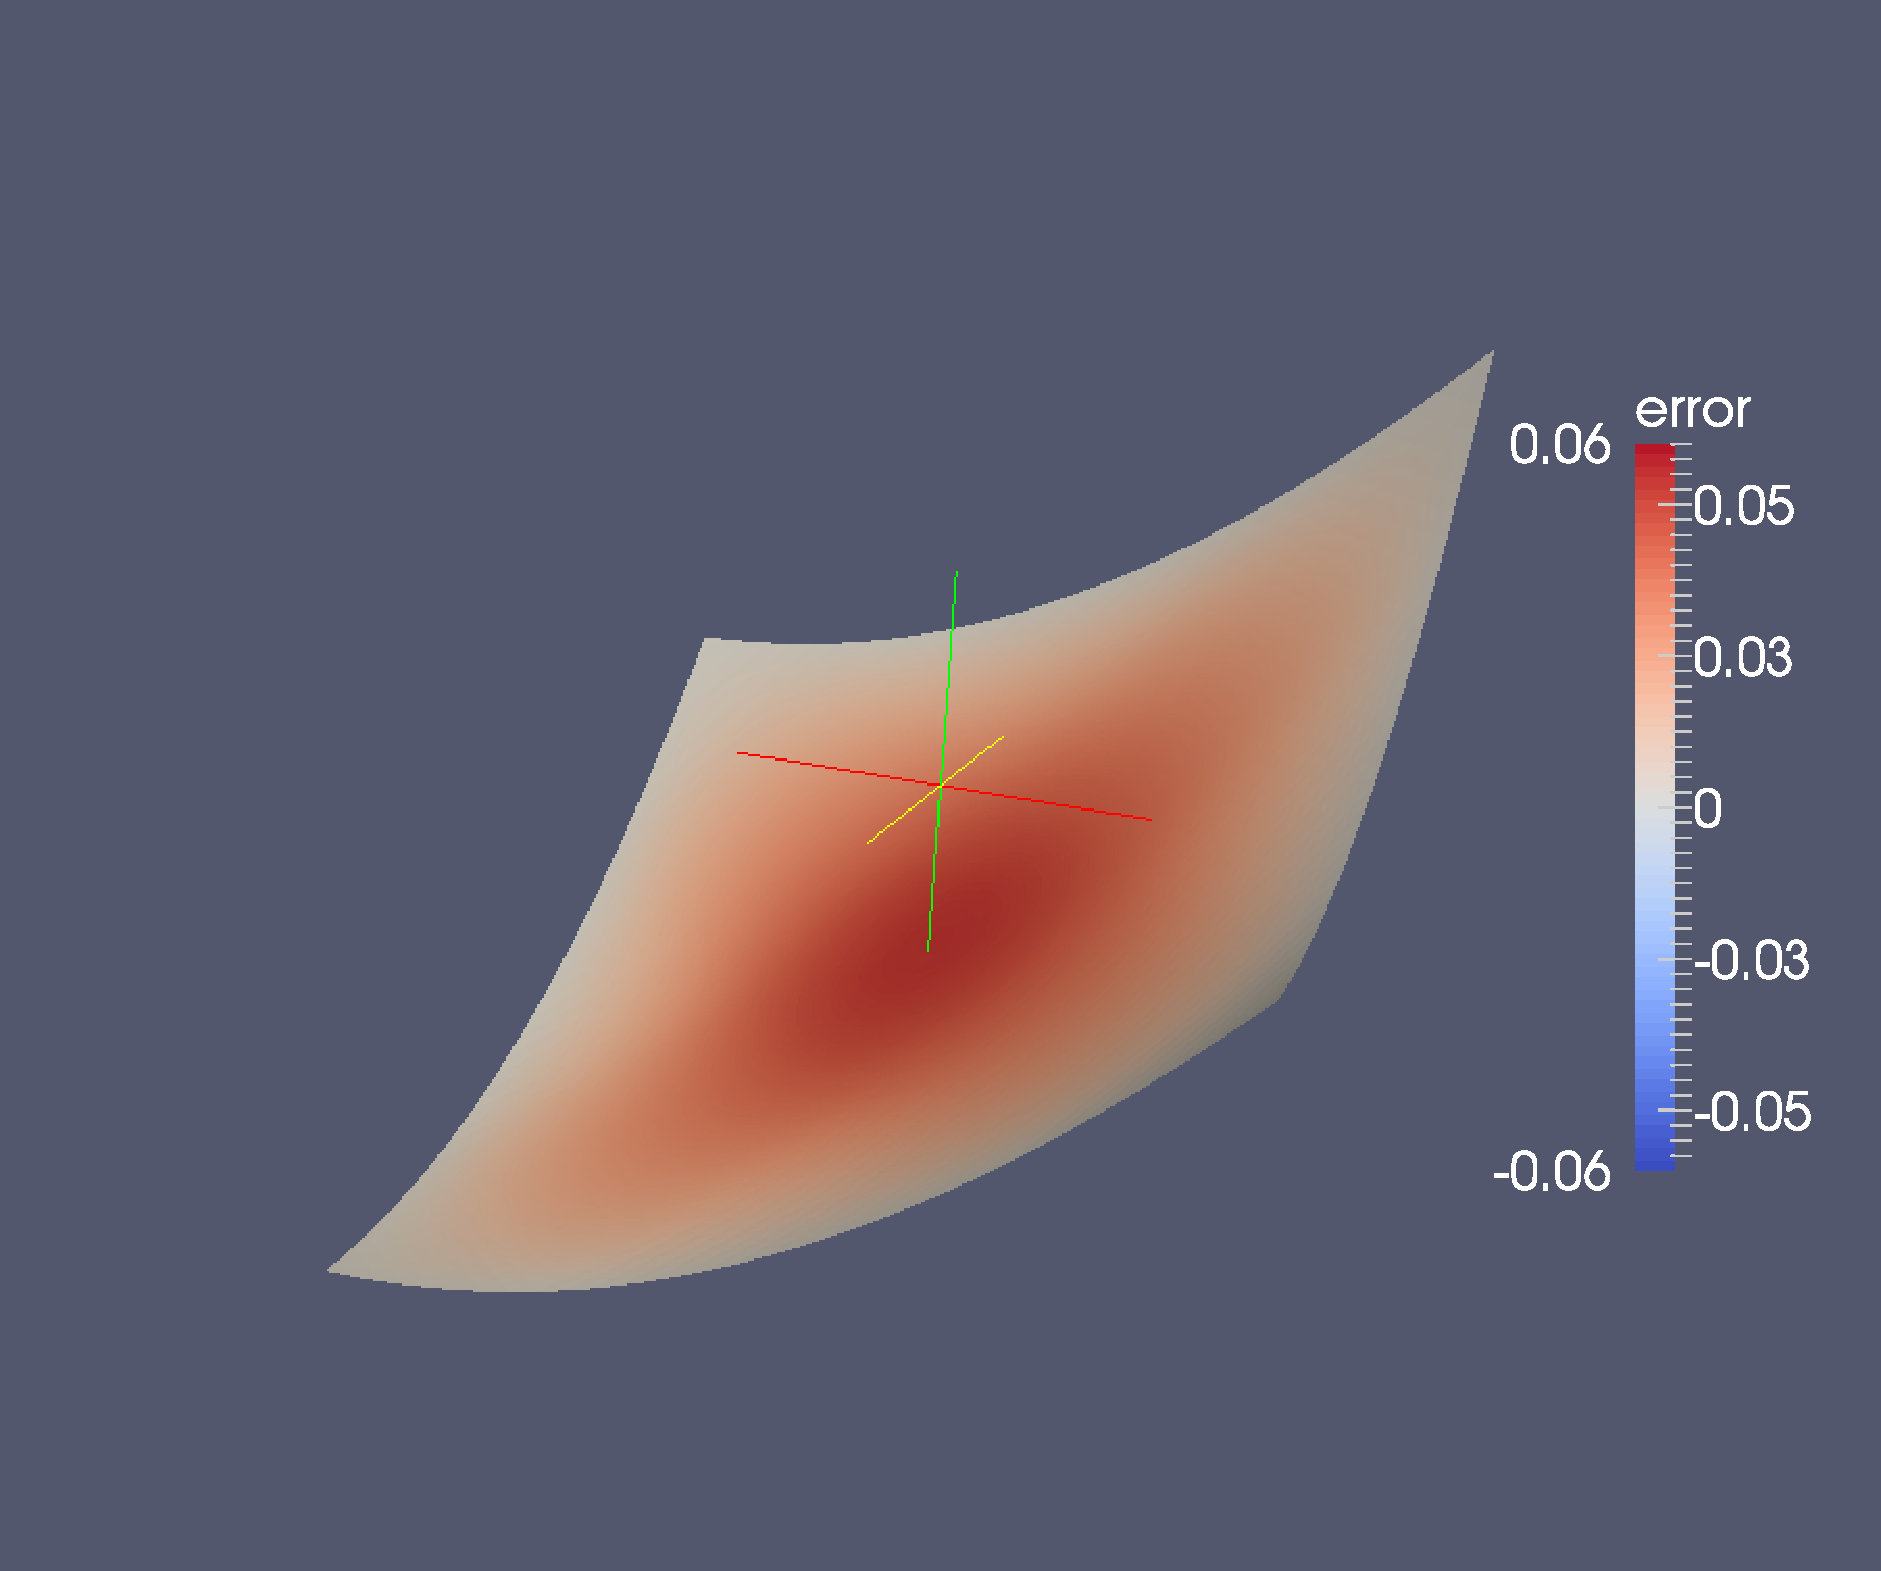
\includegraphics[width=1.\textwidth]{plots/with_penalty_it22.pdf}
	\caption{Solution after 23 steps}
\end{subfigure}
\begin{subfigure}[b]{.5\textwidth}
	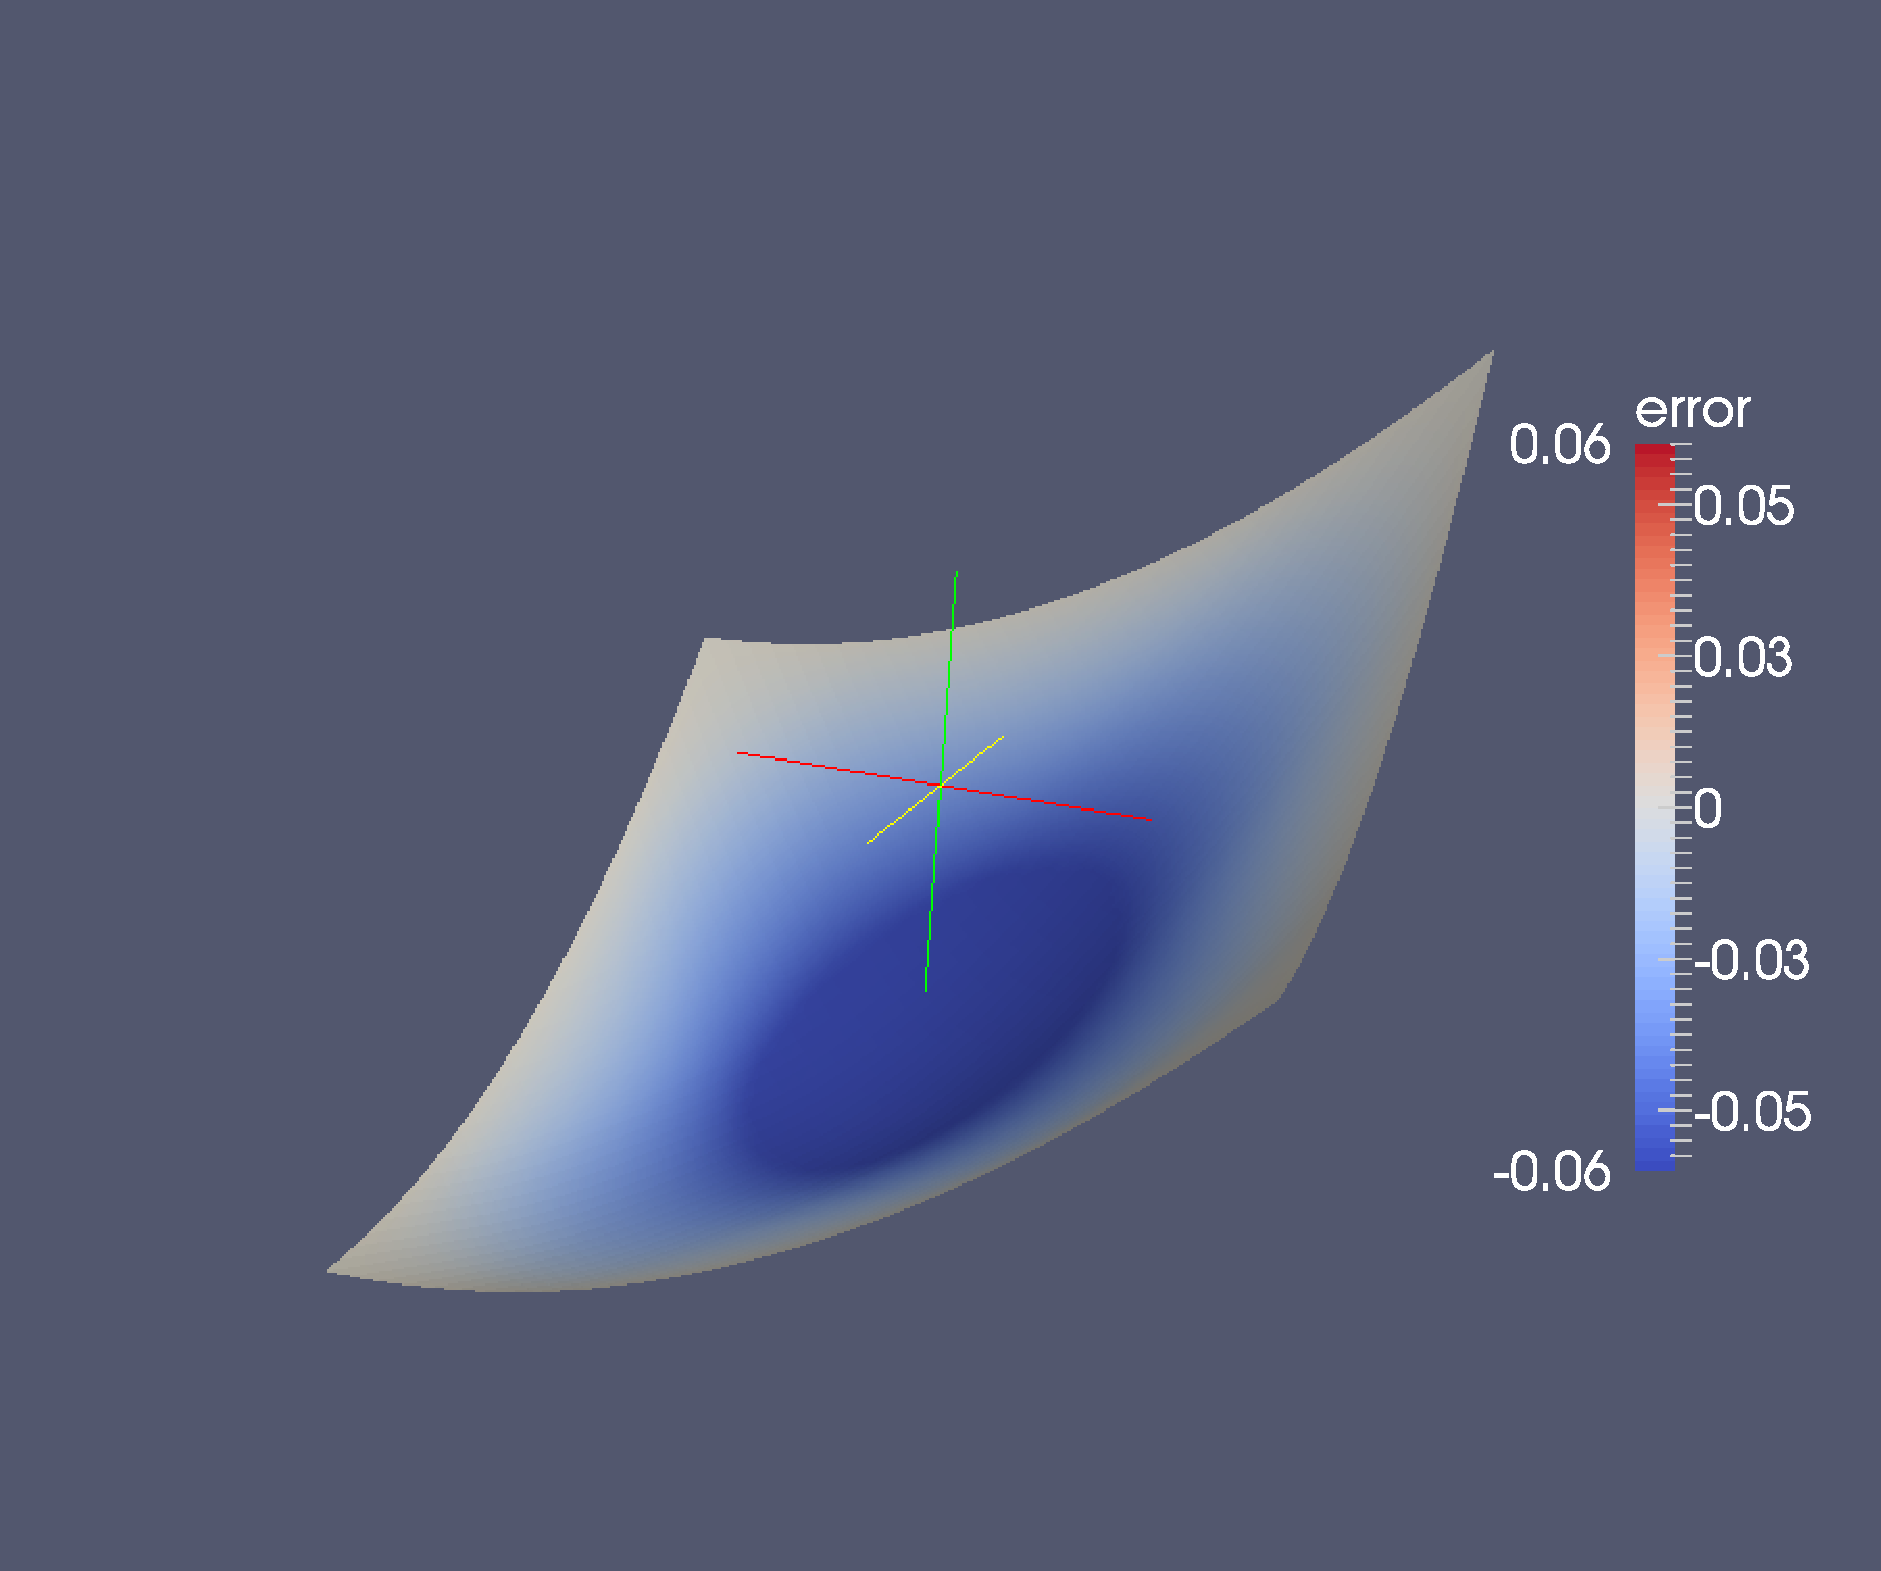
\includegraphics[width=1.\textwidth]{plots/with_penalty_it23.pdf}
	\caption{Solution after 24 steps}
\end{subfigure}
\caption{The solution in two consecutive iterations}
\label{fig: diff iteration}
\end{figure}
Figure \ref{fig: diff iteration} shows to consecutive steps, the error $u-u_{exact}$ is denoted by the surface color. We see that the solution after 23 steps lies above of the exact solution, while one iteration later the Poisson solution lies below of it. These frames are exemplary for the behaviour of our numerical solution. After a step above the solution one below follows, it looks like the solution is split into two subsequences.  And as we have also seen in the devolution of the error, these subsequences seem even to drive each other away from the actual solution.

To prevent our algorithm from doing so we couple the two subsequences by a damping. Before we continue iterating we combine the current solution with the function calculated one step before by an affine composition. Hence we got a further parameter $\alpha$, namely the amount with that the new solution contributes to the iteration.

\subsection{Modification of the Cofactor Matrix}\label{sec: mod cofactor}
For the condition of the problem it is necessary that the eigenvalues of the diffusion matrix, namely $\mycof{D_h^2 u_h^i}$ are positive for all $x$. Even better is if they are constrained from below with some constant $\varepsilon$. 
To suffice this criteria we introduce a modified cofactor matrix
\[ 
	\mycofMod {D^2_h u_h} = \begin{cases}
	\mycof {D^2_h u_h} & \lambda \geq \varepsilon	\\
	\mycof {D^2_h u_h}+ (-\lambda+\varepsilon) Id%\begin{pmatrix} -\lambda+\varepsilon & 0 \\ 0 & -\lambda+\varepsilon \end{pmatrix} 
	& else
	\end{cases}
\]
where $\lambda$ is the minimal eigenvalue of $ \mycof {D^2_h u_h}$ and $Id$ is the $d \times d$-Identity matrix. Now we replace all occurrences of $\mycof {D^2_h u_h}$ in \eqref{eq: sipg iteration} by $\mycofMod {D^2_h u_h}$ to stabilise the problem condition.

\section{The Algorithm}

Bringing those points together our method to carry out the fixed point iteration works as Algorithm \ref{alg: final} describes.

\begin{algorithm}
\begin{algorithmic}
\Require triangulation \triang, desired mesh width $h$, maximimal number of intermediate steps $i_{max}$
\State $u_0\gets $ solution of  $
	\triangle u = \sqrt{2f} \text{ in } \Omega $ with $
	u = g \text{ on }\partial \Omega$
\While {$h < H$}
	\State $i \gets 0$
%	\While {$|u_i-u_{i-1}| < \varepsilon$}
	\While {$i < i_{max} $}
		\State $u_i \gets$ solution of \ref{sec: SIPG} with modified cofactor matrix (\ref{sec: mod cofactor})
		\State $u_i \gets \alpha u_{i-1} + (1-\alpha)u_i $
		\State (convexify)
		\State $i \gets i+1$
	\EndWhile
	\State $h, \triang \gets h/2, \triangFine$
\EndWhile
\end{algorithmic}
\caption{Final Algorithm}
\label{alg: final}
\end{algorithm}

The step convexify is put into brackets for it is not clear whether a convexification is necessary and actually helps the convergence. A lot of the methods mentioned in the chapters \ref{ch:MongeAmpereEq} and \ref{ch:DGMongeAmpere} work without an explicit convexification, although most require a convex initial guess. 
Additionally the approach described in section \ref{subsec: convexification} is intricately to implement, increases significantly the computation costs and it may modify functions even though they already are convex. We note, that for the condition of the stiffness matrix of the used SIPG method we need the cofactor matrix to be positive definit which is equivalent to the piecewise convexity of the last iteration step. However, our modification of the cofactor matrix  may avert the problems arising for slightly non convex intermediate solutions.


\chapter{Numerical Results}
\label{ch:NumericalResults}
\section{Benchmark Examples}

Since the \MA equation became a benchmark problem for fully nonlinear second order PDEs there are same classical test problems for the two-dimensional case. All test cases are solved on the unitsquare $\Omega=[0,1]^2$.

\begin{test} \label{test smooth}
The first classical \MA test is the problem with the data
\[
	u=\exp( \lVert x \rVert_2^2  /2) 
	\text { and } 
	f = (1 + \lVert x \rVert_2^2) \exp( \lVert x \rVert^2).
\]
It has a very smooth solution and is even radial.

\end{test}

\begin{test}\label{test sqrt}
The data
\[
	u = - \sqrt{ 2-  \lVert x \rVert_2^2}
	\text { and } 
	f = 2\left( 2-  \lVert x \rVert_2^2 \right)^{-2}
\]
defines the second example. This test is especially interesting because the convex viscosity solution is only contained in $W^{1,p}(\Omega) $ for $p \in [0,4)$\cite{DG2006a}, i.e. it lacks $H^2$ regularity.
\end{test}

For the next two tests we define $x_0 = \left(\frac 1 2, \frac 1 2  \right)^t$.

\begin{test}\label{test singularity}
The third \MA test is yet more regular. Its solution lies in $C^1$ and it is given by
\[
	u=\frac 1 2 \left( \max 0 {\lVert x - x_0 \rVert_2-0.2 }  \right)^2 
	\text { and } 
	f = \max 0 {1-\frac {0.2} {\lVert x - x_0 \rVert_2} }.
\]
\end{test}


\begin{test}\label{test dirac}
A test determined by
\[
	u = \lVert x - x_0 \rVert_2
	\text { and } 
	f = \pi \delta_{x_0}
\]
describes a cone with origin $x_0$. Note, $f$ is highly non regular. This example does not have a viscosity solution, but $u$ is only an Aleksandrov solution of the problem \cite[Section 2.3.]{FO2011}.
\end{test}


\begin{test}\label{test rhsConst}
A test where the analytical solution is unknown is determined by
\[
	u = 0 \text{ on } \partial \Omega
	\text { and } 
	f = 1
\]
defines the last example.
\end{test}

\section{Numerical Results of a $C^0$ Penalty Method}

%read data for case deg=22 and merge into one file

\newcommand{\readData}[2]{
	\pgfplotstableread{data/#1_l2errornorm} #2
	
	\pgfplotstablecreatecol[copy column from table={data/#1_h1errornorm}{h1error}] {h1error} #2
	
	\pgfplotstablecreatecol[copy column from table={data/#1_newtonSteps}{steps}] {N} #2
}

\newcommand{\readDataO}[2]{
	\pgfplotstableread{data/#1_l2errornorm} #2
	
	\pgfplotstablecreatecol[copy column from table={data/#1_h1errornorm}{h1error}] {h1error} #2
	
	\pgfplotstablecreatecol[copy column from table={data/#1_newtonSteps}{steps}] {N} #2
}



\readData{MA1_Brenner_deg2}{\MAOneBrennerTwo}
\readData{MA1_Brenner_deg3}{\MAOneBrennerThree}
%
\readData{MA3_Brenner_deg2}{\MAThreeBrennerTwo}
%
\readData{MA4_Brenner_deg2}{\MAFourBrennerTwo}
\readData{MA4_Brenner_deg3}{\MAFourBrennerThree}


\readData{MA1_Neilan_GradJump_deg22}{\MAOneJumpdegTwoTwo}
\readData{MA1_Neilan_GradJump_deg20}{\MAOneJumpdegTwoZero}
\readData{MA1_Neilan_GradJump_deg33}{\MAOneJumpdegThreeThree}
\readData{MA1_Neilan_GradJump_deg32}{\MAOneJumpdegThreeTwo}

\readData{MA1_Neilan_deg33}{\MAOnedegThreeThree}
\readData{MA1_Neilan_deg32}{\MAOnedegThreeTwo}

\readData{MA2_Neilan_deg22}{\MATwodegTwoTwo}
\readData{MA2_Neilan_deg33}{\MATwodegThreeThree}
\readData{MA2_Neilan_GradJump_deg22}{\MATwoJumpdegTwoTwo}
\readData{MA2_Neilan_GradJump_deg33}{\MATwoJumpdegThreeThree}

\readData{MA3_Neilan_deg22}{\MAThreedegTwoTwo}
%\readDataN{MA3_Neilan_deg33}{\MAThreedegThreeThree}
\readData{MA3_Neilan_GradJump_deg10}{\MAThreeJumpdegOneZero}
\readData{MA3_Neilan_GradJump_deg22}{\MAThreeJumpdegTwoTwo}
\readData{MA3_Neilan_GradJump_deg20}{\MAThreeJumpdegTwoZero}
\readData{MA3_Neilan_GradJump_deg33}{\MAThreeJumpdegThreeThree}

\readData{MA4_Neilan_GradJump_deg10}{\MAFourJumpdegOneZero}
\readData{MA4_Neilan_GradJump_deg22}{\MAFourJumpdegTwoTwo}
\readData{MA4_Neilan_GradJump_deg33}{\MAFourJumpdegThreeThree}


%\pgfplotstableread{../../FEniCS/data/MA1_Neilan_deg22_l2errornorm} \MAOnedegTwoTwoL
%\pgfplotstableread{../../FEniCS/data/MA1_NeilanGradJump_deg22_l2errornorm} \MAOneJumpdegTwoTwo
%\pgfplotstableread{../../FEniCS/data/MA1_NeilanGradJump_deg22_h1errornorm}\MAOneJumpdegTwoTwoH

%\pgfplotstablecreatecol[copy column from table={../../FEniCS/data/MA1_NeilanGradJump_deg22_h1errornorm}{h1error}] {h1error} \MAOneJumpdegTwoTwo
%\pgfplotstablecreatecol[copy column from table={../../FEniCS/data/MA1_NeilanGradJump_deg22_newtonsteps}{steps}] {N} \MAOneJumpdegTwoTwo


For reference I implemented the algorithm introduced in Section \ref{sec: Brenner method}.
We implemented their presented method using the finite element tool FEniCS \cite{FEniCS}, the Code is append in Appendix. 
To create our initial guess I did not use a vanishing moment method as Brenner suggested, but the solution of $\triangle u = -\sqrt{2f}$ as introduced in \ref{sec: initial guess}. 

I solved the arising nonlinear system of equations with PETSc' basic line search Newton method. 
The results can be found in figure \ref{fig: Brenner test1} and in table \ref{tab: l2 errors test 1 Brenner} where $h$ denotes the grid width and $N$ denotes the iterations needed to reach the desired tolerance. 

\begin{table}[h]
	\begin{subtable}[b]{0.45\textwidth}
		\centering
%		\pgfplotstabletypeset[columns={iterations, l2error, h1error,N},
%				    every row 0 column 0/.style={set content=init},
%		]\MAOneBrennerTwo
    	\caption{Error for $k=2$}
   \end{subtable}
   ~
	\begin{subtable}[b]{0.45\textwidth}
		\centering
%		\pgfplotstabletypeset[columns={iterations, l2error, h1error,N},
%				    every row 0 column 0/.style={set content=init},
%		]\MAOneBrennerThree
 	\caption{Error for $k=3$}
	\end{subtable}
	\caption{Errors for test case \ref{test smooth}}
	\label{tab: l2 errors test 1 Brenner}
\end{table}
\begin{figure}[h!]
\centering
	\includegraphics[scale=0.35]{../../FEniCS/diagrams/MA1_Brenner_l2.pdf}
	\caption{$L^2$ errors for test case \ref{test smooth}}
	\label{fig: Brenner test1}
\end{figure}
Fitting the data we can calculate then convergence order  $2.576$ for $k=2$ and $3.306$ for $k=3$.

For the second test case the Newton did not even on the coarsest grid converge. Also in the third test case our Newton solver had problems. You can see results of the runs for $h=1/2, \dots, 1/16$ in table \ref{tab: l2 errors test 3 Brenner}, for finer grid the solver did not converge. My attempts to solve this example with FEniCS' built in damped Newton method with different relaxation parameters did also not succeed on any grid finer than $1/16$.
\begin{table}[h]
		\centering
%		\pgfplotstabletypeset[columns={iterations, l2error, h1error,N},
%				    every row 0 column 0/.style={set content=init},
%		]\MAThreeBrennerTwo
    	\caption{Error for $k=2$}
	\caption{Errors for test case \ref{test singularity}}
	\label{tab: l2 errors test 3 Brenner}
\end{table}

The fourth example does not have not a classical solution. As in the previous cases the method does not converge. The corresponding results are shown in table \ref{tab: l2 errors test 4 Brenner}.

\begin{table}[h]
	\begin{subtable}[b]{0.45\textwidth}
		\centering
%		\pgfplotstabletypeset[columns={iterations, l2error, h1error,N},
%				    every row 0 column 0/.style={set content=init},
%				    columns/l2error/.style={ /pgf/number format/sci precision=6}     % print 14 digits
%		]\MAFourBrennerTwo
    	\caption{Error for $k=2$}
   \end{subtable}
   ~
	\begin{subtable}[b]{0.45\textwidth}
		\centering
%		\pgfplotstabletypeset[columns={iterations, l2error, h1error,N},
%				    every row 0 column 0/.style={set content=init},
%				    columns/l2error/.style={ /pgf/number format/sci precision=6}     % print 14 digits
%		]\MAFourBrennerThree
 	\caption{Error for $k=3$}
	\end{subtable}
	\caption{Errors for test case \ref{test dirac}}
	\label{tab: l2 errors test 4 Brenner}
\end{table}

For the last test case with constant right-hand side and zero Dirichlet boundary data Newton's method only converged on the coarsest grid such that we cannot make any statement on this test.

We see that this method behaves well for smooth solutions. This method was designed to detect classical solutions and indeed to solve problems with non smooth solution and viscosity solutions the method is inappropriate.

\newpage
\section{Numerical Results of a Finite Element Method based on a Disrete Hessian}

I also implemented the algorithm introduced in Section \ref{sec: FEM discrete Hessian}.
Additional to the numerical results Neilan presented it is interesting to explore what happens if we vary the polynomial degree for the Hessian ansatz space. 

The implementation was also done with the Finite Element Tool FEniCS \cite{FEniCS}, the corresponding source code can be found in the appendix \ref{app: Code Neilan}. \\
The uniform triangulation $\triang$ was obtained as also explained in \ref{subsec: refinement and base cells}: First the domain was split into four triangles by drawing both diagonals and afterwards each triangle was successively divided into four congruent triangles. \\
Different to the initial guess suggested in \cite{Neilan2014} I used the solution of $\triangle u = -\sqrt{2f}$ as introduced in \ref{sec: initial guess}. All results presented base on discontinuous ansatz spaces, namely piecewise polynomial spaces as introduced in \ref{def: piecewise polySpace}.
We denote the degree of the trial space $V_h=\mathcal P_h^k$ by $k$ and the degree chosen for the Hessian ansatz space $\Sigma_h = [\mathcal{P}_h^{k_{DH}}]^{d \times d}$ by $k_{DH}$. The nonlinear system of equations given by \eqref{eq: neilan eq1} and \eqref{eq: discrete hessian} or \eqref{eq: neilan eq1 + jump} and \eqref{eq: discrete hessian}, respectively was solved with PETSc' basic line search Newton method. 
%SNES Object: 1 MPI processes
%  type: newtonls
%  SNES has not been set up so information may be incomplete
 % maximum iterations=10, maximum function evaluations=2000
 % tolerances: relative=1e-09, absolute=1e-08, solution=1e-16
  %total number of linear solver iterations=0
  %total number of function evaluations=0
  %SNESLineSearch Object:   1 MPI processes
   % type: bt
    %  interpolation: cubic
   %   alpha=1.000000e-04
  %  maxstep=1.000000e+08, minlambda=1.000000e-12
 %   tolerances: relative=1.000000e-08, absolute=1.000000e-15, lambda=1.000000e-08
  %  maximum iterations=40
  %KSP Object:   1 MPI processes
    %type: preonly
    %maximum iterations=10000, initial guess is zero
   % tolerances:  relative=1e-05, absolute=1e-50, divergence=10000
   % left preconditioning
   % using DEFAULT norm type for convergence test
  %PC Object:   1 MPI processes
  %  type: lu
  %  PC has not been set up so information may be incomplete
    %  LU: out-of-place factorization
   %   tolerance for zero pivot 2.22045e-14
   %   matrix ordering: nd
   % linear system matrix = precond matrix:
   % Matrix Object:     1 MPI processes
    %  type: seqaij
    %  rows=112, cols=112
    %  total: nonzeros=2744, allocated nonzeros=2744
    %  total number of mallocs used during MatSetValues calls =0
      %  using I-node routines: found 80 nodes, limit used is 5

Most parameters were set to the default PETSc values %which includes the solver uses cubic backtracking 
but the absolute tolerance was adjusted to $1e-8$ and the number of maximum iteration was restricted to 100. 

Figure \ref{fig: l2 errors test 1} shows the $L^2$ error of all performances of the first test case that have converged, the polynomial degrees $k$ were taken to be $1,\dots,3$ and $k_{DH}$ equal to all variants $0, \dots, k$. In Figure \ref{fig: h1 errors test 1} the corresponding $H^1$ errors are plotted.
\begin{figure}[H]
\centering
	\includegraphics[scale =0.4]{../../FEniCS/diagrams/MA1_Neilan_l2.pdf}
	\caption{$L^2$ errors for test case \ref{test smooth}}
	\label{fig: l2 errors test 1}
\end{figure}
\begin{figure}[H]
\centering
	\includegraphics[scale =0.4]{../../FEniCS/diagrams/MA1_Neilan_h1.pdf}
	\caption{$H^1$ errors for test case \ref{test smooth}}
	\label{fig: h1 errors test 1}
\end{figure}

Due to the large number of degree of freedoms the I could not obtain any results for the cases $k=2,3$ and $k_{DH}=2,3$ on the finest grid, for $k=3$ and $k_{DH}=3$ even on a mesh with $h=1/64$ the requested memory was too much.

As also experienced by Neilan the method does not work for the polynomial degree $k=1$. Similarly, in runs with a low polynomial degree $k_{DH}$ Newton's method did not converge. \todo{LU hat nicht funktioniert}
The results for the runs with $k=3$ are shown more detailed in Table \ref{tab: l2 errors test 1 deg 2}, in both tables the column $N$ refers to the number of iterations the Newton solver needed to reach the desired tolerance. 
\begin{table}[H]
	\begin{subtable}[b]{0.45\textwidth}
		\centering
		\pgfplotstabletypeset[columns={iterations, l2error, h1error,N},
				    every row 0 column 0/.style={set content=init},
		]\MAOnedegThreeThree
    	\caption{Error for $k=3, k_{DH}=3$}
   \end{subtable}
   ~
	\begin{subtable}[b]{0.45\textwidth}
		\centering
		\pgfplotstabletypeset[columns={iterations, l2error, h1error,N},
				    every row 0 column 0/.style={set content=init},
		]\MAOnedegThreeTwo
 	\caption{Error for $k=3, k_{DH}=2$}
	\end{subtable}
	\caption{Errors for test case \ref{test smooth}}
	\label{tab: l2 errors test 1 deg 2}
\end{table}
Considering this results in the smooth test scenario we observe that the error almost do not alter for different polynomial degrees $k_{DH}$ if both converge. Albeit for fine grids the methods with less difference between the two degrees seem to perform better. The calculated numerical orders as shown in table \ref{tab: order} supports this first intuition.

\begin{table}[H]
\begin{subtable}[b]{0.45\textwidth}
\centering
	\pgfplotstabletypeset
	{
		k $k_{DH}$ {numerical order}
		2 1  1.50338
		2 2  2.24427
		3 2 2.63597
		3 3 3.64758
	}
	\caption{numerical order in $L2$ norm}
\end{subtable}
\begin{subtable}[b]{0.45\textwidth}
	\pgfplotstabletypeset
	{
		k $k_{DH}$ {numerical order}
		2 1  1.65382 
		2 2  1.973
		3 2 2.39616
		3 3 2.97876
	}
	\caption{numerical order in $H1$ norm}
	\end{subtable}
\caption{numerical order in test \ref{test smooth}}
\label{tab: order}
\end{table}

This test scenario was also performed with the additional normal jump penalty term as stated in \eqref{eq: neilan eq1 + jump} weighted with $\eta$ equal to 50 leading to the results shown in figure \ref{fig: l2 errors test 1 jump} and the tables \ref{tab: l2 errors test 1 deg 2 jump}.

\begin{figure}[h!]
\centering
	\includegraphics[scale=0.4]{../../FEniCS/diagrams/MA1_Neilan_GradJump_l2.pdf}
	\caption{$L^2$ errors for test case \ref{test smooth} and additional gradient jump penalty}
	\label{fig: l2 errors test 1 jump}
\end{figure}

\begin{figure}[H]
\centering
	\includegraphics[scale =0.4]{../../FEniCS/diagrams/MA1_Neilan_GradJump_h1.pdf}
	\caption{$H^1$ errors for test case \ref{test smooth} and additional gradient jump penalty}
	\label{fig: h1 errors test 1 jump}
\end{figure}
\begin{table}[H]
	\begin{subtable}[b]{0.45\textwidth}
		\centering
		\pgfplotstabletypeset[
		columns={iterations, l2error, h1error,N},
		    every row 0 column 0/.style={set content=init},
		    every row 7 column 1/.style={set content={-}},
		    every row 7 column 2/.style={set content={-}},
		    every row 7 column 3/.style={set content={-}},
		]\MAOneJumpdegTwoTwo
    	\caption{Error for $k=2, k_{DH}=2$}
   \end{subtable}
   ~
	\begin{subtable}[b]{0.45\textwidth}
		\centering
		\pgfplotstabletypeset[columns={iterations, l2error, h1error,N},
		    every row 0 column 0/.style={set content=init},
		]\MAOneJumpdegTwoZero
	\caption{Error for $k=2, k_{DH}=0$}
	\end{subtable}
	\caption{Errors for test case \ref{test smooth}}
	\label{tab: l2 errors test 1 deg 2 jump}
\end{table}
As claimed by Neilan the additional penalisation leads to a convergend method even for low polynomial degrees, even in the cases where only $k_{DH}$ was taken to be small. The calculated error norms indicate more clearly than in the non penalised runs that variation of $k_{DH}$ yields only to a slight loss of accuracy. The corresponding numerical orders can be found in \ref{tab: order jump}.
\begin{table}[H]
\centering
\begin{subtable}[b]{0.45\textwidth}
	\pgfplotstabletypeset
	{
		k $k_{DH}$ {numerical order}
		1 0 1.32061
		2 0 2.69871
		2 1 2.93488
		2 2 3.0406
		3 1 3.63116
		3 2 4.01895
		3 3 4.0588
	}
	\caption{numerical order in $L2$ norm}
	\end{subtable}
	\begin{subtable}[b]{0.45\textwidth}
	\pgfplotstabletypeset
	{
		k $k_{DH}$ {numerical order}
		1 0 0.978853
		2 0 2.24561
		2 1 2.24836
		2 2 2.28606
		3 1 3.03434
		3 2 3.0359
		3 3  3.0343
	}
	\caption{numerical order in $H1$ norm}
	\end{subtable}
	\caption{numerical order with jump penalty in test \ref{test smooth}}
\label{tab: order jump}
\end{table}


The second test two was carried out for $\eta=20k^2$. Unfortunalety the Newton solver did not converge after the mesh was once refined. Table \ref{tab: l2 errors test 2} show the results for this one step, it shows only two degree pairs for other degree paris behaved similarly.

%\begin{figure}[H]
%\centering
%	\includegraphics[scale =0.4]{../../FEniCS/diagrams/MA2_Neilan_l2.pdf}
%	\caption{$L^2$ errors for test case \ref{test sqrt} }
%	\label{fig: l2 errors test 2}
%\end{figure}

\begin{table}[H]
	\begin{subtable}[b]{0.45\textwidth}
		\centering
%		\pgfplotstabletypeset[
%		columns={iterations, l2error, h1error,N},
%		    every row 0 column 0/.style={set content=init},
%		]{\MATwodegTwoTwo}
    	\caption{Error for $k=2, k_{DH}=2$}
   \end{subtable}
   ~
	\begin{subtable}[b]{0.45\textwidth}
		\centering
%		\pgfplotstabletypeset[columns={iterations, l2error, h1error,N},
%		    every row 0 column 0/.style={set content=init},
%		]{\MATwodegThreeThree}
	\caption{Error for $k=3, k_{DH}=3$}
	\end{subtable}
	\caption{Errors for test case \ref{test sqrt}}
	\label{tab: l2 errors test 2}
\end{table}

Switching the penalisation of gradient jumps on the method performs again well, its results are shown in figure \ref{fig: l2 errors test 2 jump}. 

\begin{figure}[H]
\centering
\begin{subfigure}{\textwidth}
\centering
	\includegraphics[scale =0.4]{../../FEniCS/diagrams/MA2_Neilan_GradJump_l2.pdf}
\end{subfigure}

\begin{subfigure}{\textwidth}
\centering
	\includegraphics[scale =0.4]{../../FEniCS/diagrams/MA2_Neilan_GradJump_h1.pdf}
\end{subfigure}
	\caption{$L^2$ and $H^1$ errors for test case \ref{test sqrt} and additional gradient jump penalty}
	\label{fig: l2 errors test 2 jump}
\end{figure}

Similar are results for the third case, but now also an additional penalisation of the jump of the gradient across edges do not yield to better results. All converged iteration steps are given in the tables \ref{tab: l2 errors test 3} and \ref{tab: l2 errors test 3 jump}. 

\begin{table}[H]
	\begin{subtable}[b]{0.45\textwidth}
		\centering
%		\pgfplotstabletypeset[
%		columns={iterations, l2error, h1error,N},
%		    every row 0 column 0/.style={set content=init},
%		]{\MAThreedegTwoTwo}
    	\caption{Error for $k=2, k_{DH}=2$}
   \end{subtable}
   ~
	\begin{subtable}[b]{0.45\textwidth}
		\centering
%		\pgfplotstabletypeset[columns={iterations, l2error, h1error,N},
%		    every row 0 column 0/.style={set content=init},
%		]{\MAThreedegThreeThree}
	\caption{Error for $k=3, k_{DH}=3$}
	\end{subtable}
	\caption{Errors for test case \ref{test singularity}}
	\label{tab: l2 errors test 3}
\end{table}


\begin{table}[H]
	\begin{subtable}[b]{0.45\textwidth}
		\centering
		\pgfplotstabletypeset[
		columns={iterations, l2error, h1error,N},
		    every row 0 column 0/.style={set content=init},
		]{\MAThreeJumpdegTwoTwo}
    	\caption{Error for $k=2, k_{DH}=2$}
   \end{subtable}
   ~
	\begin{subtable}[b]{0.45\textwidth}
		\centering
		\pgfplotstabletypeset[columns={iterations, l2error, h1error,N},
		    every row 0 column 0/.style={set content=init},
		]{\MAThreeJumpdegThreeThree}
	\caption{Error for $k=3, k_{DH}=3$}
	\end{subtable}
	\caption{Errors for test case \ref{test singularity} and additional gradient jump penalty}
	\label{tab: l2 errors test 3 jump}
\end{table}


%\begin{figure}[H]
%\centering
%\begin{subfigure}{\textwidth}
%	\includegraphics[scale =0.4]{../../FEniCS/diagrams/MA3_Neilan_GradJump_l2.pdf}
%\end{subfigure}
%	\caption{$L^2$ and $H^1$ errors for test case \ref{test sqrt} and additional gradient jump penalty}
%	\label{fig: l2 errors test 3 jump}
%\end{figure}


\newpage

\section{Numerical Results of Our DG Method}

Our method was implemented in pure C++. The underlying grid structure was taken from the implementation of \cite{BMV2009}, handling vectors and matrices as well as was linear solver were provided by the Eigen library \cite{eigenweb}. To solve the quadratic program arising in the context of convexification the C++ library ipopt \cite{ipopt} was used.

\todo{mesh}

\subsection{Implementation Details}

The main class of the implementation is the Tsolver class. Here come all information together and the solver controls the assembly and solving process. 
We make the clear looking at a . The main method can be found in mesh.cpp. At the beginning all input data is fed into the program. With this information the solver can initialise the grid and the reference cell. 
The grid is taken from the igpm\_t2\_lib and based on the work of \cite{BMV2009} and all reference data is handled in the class Tshape.

\subsubsection{alternative 1}
The main work is done in Tsolver's function stepping\_MA(). It starts with an initialisation process where it reads specific problem data which includes
\begin{enumerate}
 \item  the problem we want to solve,
 \item penalty parameters to enforce continuity and penalise the gradient jump,
 \item the start level of refinement with respect to the initial grid,
 \item the damping paramter alpha,
 \item the number of fixed point iterations per grid,
 \item the maximal grid refinements.
\end{enumerate}
During the initialisation it also updates all base cell data, the leaf cell data, enumerate the degree of freedoms and the initial guess.
Afterwards the fixed point iterations begin, in every step the General Poisson Problem is solved, eventually convexified and afterwards with the last solution step combined. If the specified number of iterations has been carried out, the grid is refined, the leaf cell data updated and we start the fixed point iterations again.
We repeat this process until the maximal number of grid refinements is reached.


\subsubsection{alternative 2}
The main work is done in Tsolver's function stepping\_MA(). Algorithm \ref{alg: stepping} illustrates how this function works.
\begin{algorithm}[H]
\begin{algorithmic}
	\State Read problem specific data:
		\begin{enumerate}
			 \item  problem\_name \Comment {to choose right-hand side and boundary conditions}
			 \item penalty parameters   \Comment {  to enforce continuity and penalise the gradient jump}
			 \item start\_level  \Comment { the start level of refinement with respect to the input grid}
			 \item $\alpha$  \Comment {the damping paramter}
			 \item maxits \Comment{ the number of fixed point iterations per grid}
			 \item max\_levelrefinement \Comment{ the maximal refinement level }
		\end{enumerate}
	\State Initialise base cell data
	\State Refine to start\_level
	\State Initialise leaf cell data
	\State Enumerate degree of freedoms
	\State (Initialise Convexifier)
	\State Initialise initial guess $u_{-1}$
	\State $i \gets 0$
	\While {level < max\_levelrefinement}
		\State Enumerate degree of freedoms
		\State (Initialise C0 converter) \Comment{only needed for convexification}
		\State cur\_it$ \gets 0$
		\While {cur\_it < maxits}
			\State  assemble\_MA()                              \Comment Assemble system for General Poisson Problem
			\State $u_i \gets$ solution of assembled system
			\State (Convexify $u_i$)		 
			\State $u_i \gets \alpha u_{i-1}  +(1-\alpha) u_i$
			\State	cur\_it, i $\gets$ cur\_it$+1$, i$+1$
			\State Restore\_MA() 		\Comment{Store solution in leaf cells}
		\EndWhile
		\State Refine grid and update leaf cell data
		\State level $\gets$ level $+1$
	\EndWhile
\end{algorithmic}
\caption{stepping\_MA}
\label{alg: stepping}
\end{algorithm}

Direct at the beginning of system assembly the diffusion matrix in every cell has to be updated with the current cofactor matrix of the Hessian. Note, that this matrix is constant for polynomial degree $k=2$ and otherwise has to be calculated for every quadrature point. Since in general here is no connection between diffusion matrix values at the reference cell and in the leaf cell, the values of the diffusion matrix are stored in the leaf cells.
The assembly process is carried out as already mentioned in algorithm \ref{alg: assembling}. Hereby one has to pay attention to the right scaling of quadrature weights and the right calculation of quadrature data from reference cell data as described in Examples \ref{ex: base cell trafo} and \ref{ex: leaf cell trafo}. 

If a convexification is desired the class Convexifier takes care of the assembly of the matrices $A$ and $C$ for \eqref{eq: convex lsq} and deals with ipopt's interface to solve the quadratic program.

Additionally the Tsolver has a member Plotter handling all export to files. It is able to write the solution which's coefficients are currently stored in the leaf cells to a .vtu file or .dat file. Besides plotting it also administers all file stream to which information such as $L2$ errors are written into.

\subsection{Results with Convexification}

For a initial guess I also used the solution of $\triangle u = -\sqrt{2f}$ combined with the multilevel approach as described in \ref{sec: initial guess}.
The arising linear system of equations was solved with Eigen's internal Cholesky solver.
The parameters were if not other specified taken to be $\sigma=10 k^2, \sigma_G = 50, \alpha =
0.3$ and $\varepsilon = 1e-2$. We always carry out 15 steps including a convexification after every step before we refine further. The implemented convexification followed the ideas of Section \ref{subsec: convexification}. 

The linear constraints ensuring convexity on a triangle are chosen the one from theorem \ref{thm: convex cond on triangle} and the constrains for convexity across edges were given by theorem \ref{thm: convex cond across edge}. Due to the error-proneness during the assembly of $C$ the convexification was only implement for the case $k=2$. Note, that before applying the theorems of section \ref{subsec: convexification} we have to convert our numerical solution from the DG formulation to a $C^0$ spline.

The linearly constrained least square problem \eqref{eq: convex lsq}  was reformulated as a quadratic program with linear constraints using normal equations. 
The quadratic program was solved with the C++ library ipopt \cite{ipopt}. Fortunately the evaluation matrix $A$, and the constraint matrix $C$ of \eqref{eq: convex lsq} only depend on the grid. Hence they need only to be assembled once after every refinement.


The results shown in figure \ref{fig: l2 errors test smooth ourMethodConvex} are very disillusioning.
\begin{figure}[H]
\centering
	\includegraphics[scale =0.4]{plots/MA1_convexify.pdf}
	\caption{$L^2$ errors for test case \ref{test smooth} and additional convexification}
	\label{fig: l2 errors test smooth ourMethodConvex}
\end{figure}
We plotted in figure \ref{fig: convex before after} the $L2$ errors before the convexification step and after it. As we can see the convexification process increases the error. There are several possible explanations for that:\\
Though the used convexification algorithm produces a convex result it does not garantuee that it leaves convex input functions unchanged.\\
The convex function in $\mathcal P^2_h$ approximating the numerical solution $u_h$ best is not necessarily closer to the exact solution $u$ than $u_h$. Then the convexification gives a push into the wrong direction. \\
Also the best approximation of $u$ into $\mathcal P^2_h$ does not have to be convex\todo{aguilera}. I have examined for the triangulation with $h=1/2$ the vector $Cc_u$ where $c_u$ are the coefficients of $L2$ projection into $\mathcal P^2_h$ and its minimal entry is -9.77e-03, for a grid with $h=1/16$ the minimal entry is -4.26e-04. Thus, the $L2$ projection of the exact solution does not comply with the convexity conditions.
Figure \ref{fig: convex min coeffs} plots the minimal entry of $Cc$ for every Generalised Poisson solution vector $c$. We see that especially for small grid widths the solutions do not fulfill the convexity conditions. \todo{grid structure maxima etc.}


\begin{figure}[H]
\centering
	\begin{subfigure}{0.45\textwidth}
		\includegraphics[scale=0.25]{plots/MA1_convexComp.pdf}
		\caption{Comparison of $L2$ errors directly before and after convexification}
		\label{fig: convex before after}
	\end{subfigure}
	\begin{subfigure}{0.45\textwidth}
		\includegraphics[scale=0.25]{plots/MA1_minCoeff.pdf}
		\caption{Comparison of $L2$ errors directly before and after convexification}
		\label{fig: convex min coeffs}
	\end{subfigure}	
	\caption{$L^2$ errors for test case \ref{test smooth} and additional convexification}
	\label{fig: Compare test smooth ourMethodConvex}
\end{figure}


The other test cases produce similar results as can be seen in figure \ref{fig: l2 errors test singularity ourMethodConvex} ... \todo{}

\begin{figure}[H]
\centering
	\includegraphics[scale =0.4]{plots/MA2_convexify.pdf}
	\caption{$L^2$ errors for test case \ref{test singularity} and additional convexification}
	\label{fig: l2 errors test singularity ourMethodConvex}
\end{figure}
\begin{figure}[H]
\centering
	\includegraphics[scale =0.4]{plots/MA2_convexComp.pdf}
	\caption{$L^2$ errors for test case \ref{test singularity} and additional convexification}
	\label{fig: Compare test singularity ourMethodConvex}
\end{figure}



\subsection{Results without Convexification}

We used the same code basis as in the previous tests but turned off every direct convexification.
In the first figure \ref{fig: l2 errors test smooth ourMethod} we can see the results for the the smooth test case \ref{test smooth}.
\begin{figure}[h!]
	\centering
	\includegraphics[scale =0.4]{plots/MA1.pdf}
	\caption{$L^2$ errors for test case \ref{test smooth}}
	\label{fig: l2 errors test smooth ourMethod}
\end{figure}
 For the first four refinements the method behaves well for both $k=2$ and $k=3$. Afterwards the numerical solution departs from the actual solution although the $L^2$ error seems to not excel $1$.
 
 We get similiar results in the next two cases albeit the fixed point iterations performs worse in the second case which lacks $H^2$ regularity. The $L2$ errors are shown in the figures \ref{fig: l2 errors test sqrt ourMethod} and \ref{fig: l2 errors test singularity ourMethod}.
 
\begin{figure}[H]
\centering
	\includegraphics[scale =0.4]{plots/MA3.pdf}
	\caption{$L^2$ errors for test case \ref{test sqrt}}
	\label{fig: l2 errors test sqrt ourMethod}
\end{figure}


\begin{figure}[H]
\centering
	\includegraphics[scale =0.4]{plots/MA2.pdf}
	\caption{$L^2$ errors for test case \ref{test singularity}}
	\label{fig: l2 errors test singularity ourMethod}
\end{figure}

The results were validated by a reference implementation using the finite element tool FEniCS. Albeit I was not able to include the modified cofactor matrix to the bilinear form the error behaved as in the computational results of the C++ code. It decreased for the first four refinements and diverged afterwards. 

Additionally one can in the FEniCS variant the cofactor matrix of the Hessian which is evaluated piecewise replace by the discrete Hessian as defined in \ref{def: discrete Hessian} for a symmetric ansatz space $\Sigma_h$. The code can be found in the Appendix \todo{ref}.


\chapter{Conclusion und Perspective}
\label{ch:conclusion}
\section{Comparison with Newton's method}

Before we start the anlaysis of our Method we shortly see what happens if we apply Newton's method on the analytical form of the \MA equation \ref{MA eq}.
Let $F$ be the function such that its root solves the \MA equation, i.e. 
\[
	F(u) = \mydet{D^2 u} -f
\]
Applying Newton's method on $F(u) =0$ we have
\begin{align}
	DF[u^n](u^{i+1}-u^i) = -F[u^i]
\end{align}
where $DF[u]$ denotes the G\^ateaux derivative. We derived the G\^ateaux derivative $DF[u] v = \mycof{D^2 u}:D^2v$ already in theorem \ref{thm: linearisation} leading us to the Newton iteration
\begin{align}
	\mycof{D^2 u^i}:D^2\left(u^{i+1}-u^i\right) &= -\mydet{D^2 u^i}+f \nonumber \\
	\Leftrightarrow \qquad \qquad  \mycof{D^2 u^i}:D^2(u^{i+1}) &= -\mydet{D^2 u^i} +f  +\mycof{D^2 u^i}:D^2(u^i). \label{eq: Newton iteration pre}
\end{align}

Similar to the derivation of the fixed point iteration we can apply Lemma \ref{la: An application of the divergernce product rule} to rewrite \eqref{eq: Newton iteration pre} and we have the problem
\begin{align}
	\nabla \cdot \left( \cof(D^2 u^0) \nabla u^{i+1} \right) &= -\mydet {D^2u^i} +f+\nabla \cdot \left( \cof(D^2 u^i) \nabla u^{i} \right)  \textnormal{ in } \Omega,  \label{eq: Newton iteration}\\
	u^{i+1} &= g \textnormal{ on } \partial \Omega .
\end{align}

Hence, considering once again the fact 
\[
\nabla \cdot \left( \mycof {D^2 u } \nabla v \right)
\stackrel{La.\ref{la: An application of the divergernce product rule}}=\nabla \cdot {}\mycof{D^2 u}:D^2u
=\frac 1 2 \mydet{D^2u}.
\]
we can see our method as a variant of Newton's method. 

In \cite{Awanou2014} Awanou analysed the similar iteration process
\begin{align}
	\nabla \cdot \left( \cof(D^2 u^0) \nabla u^{i+1} \right) &= \nabla \cdot \left( \cof(D^2 u^0) \nabla u^{i} \right) + f - \operatorname{det} (D^2u^i) \textnormal{ in } \Omega,  \label{eq: Awanout eq}\\
	u^{i+1} &= g \textnormal{ on } \partial \Omega.
\end{align}
showing convergence for the analytical solution $u$ and a sufficent close $u^0$. 
In a earlier work \cite{Awanou2010} Awanou examined a discrete Version of a vanishing moment method, herein he mentioned a method he calls Newton's method defined by
\[
	\int_{\Omega} [\mycof{ D^2 u_h^i} Du_h^{i+1}] \cdot Dv_h = -	\int_{\Omega} f v_h + \frac 1 2 \int_{\Omega} [\mycof{ D^2 u_h^i} Du_h^{i}] \cdot Dv_h \; \forall v_h \in V_h \cap H^1_0 (\Omega)  \label{eq: Awanout eq2}.
\]
And indeed this is the variational form of \eqref{eq: Newton iteration}
His chosen trial space were piecewise polynomials contained in $C^1(\Omega)$. He claims that this ansatz breaks down for problems with non-smooth solutions, in his numerical results he cites test \ref{test sqrt} as an example where Newton's method diverges.

\todo{existence theory}
\section{Comparison with the $C^0$ penalty method}
It is also interesting to compare our linearisation with the linearisations of the two other methods.
Consider a Newton step made in the $C^0$ penalty method (cf. \ref{sec: Brenner method}).
\begin{align}
	&\int_\Omega \cofHess {u^i} \nabla (u^{i+1}-u^i) \nabla v - \sum_{e \in \edgesb} \int_e \cofHess {u^i} \nabla (u^{i+1}-u^i) \cdot \mathbf n \; v \nonumber \\
	&- \sum_{e \in \edgesb} \int_e \cofHess {u^i} \nabla v \cdot \mathbf n (u^{i+1}-u^i) + \sigma \sum_{e \in \edgesb} \frac 1 {|e|} \int_e v (u^{i+1}-u^i)\nonumber \\
	=&-\int_\Omega \left(f - \detHess{u^i)}\right) v  
			- \sum_{e \in \edgesi} \int_e \jump { \average{\cofHess {u^i}} \nabla {u^i} } v \nonumber \\
&	- \sum_{e \in \edgesb} \int_e \cofHess {u^i} \nabla v \cdot \mathbf n \; (u^i-g) - \sigma \sum_{e \in \edgesb} \frac 1 {|e|} \int_e v (u^{i}-g) \label{eq: a newton step Brenner}
\end{align}
To compare both linearisations we first reorder and remove cancelling terms in \eqref{eq: a newton step Brenner}.
\begin{align}
	&\int_\Omega \cofHess {u^i} \nabla u^{i+1} \nabla v \\
	&- \sum_{e \in \edgesb} \int_e \cofHess {u^i} \nabla u^{i+1} \cdot \mathbf n \; v 
		- \sum_{e \in \edgesb} \int_e \cofHess {u^i} \nabla v \cdot \mathbf n \; u^{i+1} \\
	=
	&-\int_\Omega \left(f - \detHess{u^i)}\right) v \\
	&+ \sum_{e \in \edgesb} \int_e \cofHess {u^i} \nabla v \cdot \mathbf n \; g 
	+\sigma \sum_{e \in \edgesb} \frac 1 {|e|} \int_e v (-u^{i}+g) \label{eq: ordered newton step Brenner}
\end{align}

\section{Conclusion}

We saw the performances of three DG methods solving PDEs of \MA type.
The first method, introduced by Brenner et alter yields a good result for the smooth test case but failed for every other test case, even for test case \ref{test singularity} that has a solution in $C^1(\Omega)$. Hence, as the developer indicate in their paper it is only suitable for finding classical solutions.
Brenner et alter used a vanishing moment method to find a proper initial guess. This seems rather costly and our numerical results show the method could be improved using a nested iterations and a simple linear PDE for the first initial guess.

The results Neilan showed in his paper for our second examined method look very promising.
Note, that this method has if polynomial degree of $V_h$ and $\Sigma_h$ are chosen equally has as five times as many degree of freedoms compared to both other methods.

The last presented method turned out to be a variant of an classical damped Newton approach. 
\todo{verbesserung mit modifizierter cofactor matrix}
The classical approach is known to fail for elements which are not at least contained in $C^1(\Omega)$. Unfortunately the fixed point iteration do also diverge for finer grids. Yet it may serve for an initial guess during a multilevel method. For big grid widths in our test cases the $L2$ error even decreased for problems which do not have a classical solution.

Comparing the three methods for the smooth test case the first and second method produce similar convergence orders while the first has less degree of freedoms. The Picard type method yields even for the first four refinement a much smaller convergence rate.

We saw that recent DG methods perform well on problems with classical solution, but have problems with problems with only viscocity solution or Aleksandrov solutions. Most rely on Newton's method to solve their nonlinear system and how to provide good initial guesses is not answered yet.
My numerical results show that a nested iteration approach often does not provide suitable starting points for further refinements.

\section{Perspective}
Handling fully nonlinear PDEs is a complex domain and results on this domain are very unsatisfactory when compared to the linear case. Even when restrict ourselves to the prototype of nonlinear PDEs, the \MA equation, the theory is far from being complete for both the analytical and the numerical point of view.

Recent DG methods work provably well for classical solutions, but to the author's knowledge there are no proven statement on their performance for viscosity solutions or Aleksandrov solutions. Even in the case we have a classical solution convergence of DG method is only proven for polynomial degrees greater or equal than three. Though most numerical experiment suggest a relaxation it could not be proved yet.

We presented methods for the \MA equation given that the right-hand side only depend on $x$ and the left-hand side only on the determinant of the Hessian. Currently DG methods were often not extended to more general PDEs. It has to be analysed, if  discretisations for right-hand sides depending on $u$ and $\nabla u$ and more complicated left-hand sides may be derived analogously. An example for one of those more complicated left-hand sides is $\mydet {D^2 u +A}$ for $A:\Omega \rightarrow \R^{d \times d}$.
 
The implemented convexification did not support the solution process. Yet, it is worth to address this approach further. Maybe it is useful to convexify intermediate solution only on fine grids.




\newpage
%\input{literatur.tex}
% bib
\newpage
%\nocite*{} 
\bibliography{literatur.bib,my_additional_bibliography.bib}
\bibliographystyle{unsrt}
\end{document}
